%TODO some other important todos are written throughout this document, some aren't very important, some should be done before uploading

%TODO Put blocks in something like textsc or texttt, config variables in $$, etc.
%TODO change MySystem to househeat example

%TODO do web links in a standard way (currently a mix of href and url)

%TODO might use pronouns like I/we (not sure, but I'm guessing you guys don't want that). I searched for and removed contractions though

%TODO Delete/Update ...\doc\Projects\Simulink_Documentation\LEAP_SDD_Tool\Examples\sldemo_househeat & DemoModel2011b

% \documentclass[12pt,letterpaper]{report}
\documentclass{mcscert}
\docdate{July 2018}

\usepackage[utf8]{inputenc}
\usepackage{graphicx}
\graphicspath{ {figs/} }
\usepackage{hyperref}
\usepackage[]{mcode}
\usepackage{cleveref}[2012/02/15]% v0.18.4;
\usepackage{url}
\usepackage[toc,page]{appendix} 
\usepackage{subcaption}
\usepackage{bold-extra} % so that small caps can able be bolded (for the \matalb) command

\usepackage[titles]{tocloft} % needed in order to add space after toc numbers so they don't overlap with the text
\addtolength{\cftsecnumwidth}{2pt}

\usepackage{footmisc} % allow referencing footnotes

%\setcounter{secnumdepth}{4}

% --------- Block Names ---------
\usepackage{xspace}

\newcommand{\args}[1] {\textit{#1}}
\newcommand{\cmd}[1] {\texttt{#1}}     % Use for command window commands, e.g., \cmd{svn up}
\newcommand{\block}[1] {\textsf{#1}}   % Use for Simulink block names, e.g., \cmd{Subsystem1}
\newcommand{\signal}[1] {\textsf{#1}}   % Use for Simulink block names, e.g., \cmd{Subsystem1}
\newcommand{\ring}[1] {\textsf{#1}} 	 % Use for files names and paths
\newcommand{\keyword}[1] {\texttt{#1}} % Use for keywords of programming languages, e.g., \keyword{while}
\newcommand{\file}[1] {\texttt{#1}} 	 % Use for files names and paths
\newcommand{\param}[1] {\textsf{#1}}   % Use for block parameter names, e.g., \param{BlockType}

% Matlab Products
\newcommand{\matlab}{\textsc{Matlab}\@\xspace}
\newcommand{\Matlab}{\textsc{Matlab}\@\xspace}
\newcommand{\Simulink}{Simulink\@\xspace}
\newcommand{\simulink}{Simulink\@\xspace}
\newcommand{\SDV}{Simulink Design Verifier\@\xspace}
\newcommand{\mpath}{\Matlab search path\@\xspace}

% Block Names (not BlockType)
\newcommand{\ds}{\block{Data Store}\@\xspace}
\newcommand{\DSM}{\block{Data Store Memory}\@\xspace}
\newcommand{\DSR}{\block{Data Store Read}\@\xspace}
\newcommand{\DSW}{\block{Data Store Write}\@\xspace}
\newcommand{\DSRW}{\block{Data Store Read/Write}\@\xspace}
\newcommand{\DSMRW}{\block{Data Store Memory/Read/Write}\@\xspace}

\newcommand{\goto}{\block{Goto}\@\xspace}
\newcommand{\from}{\block{From}\@\xspace}

\newcommand{\inport}{\block{Inport}\@\xspace}
\newcommand{\outport}{\block{Outport}\@\xspace}
\newcommand{\constant}{\block{Constant}\@\xspace}
\newcommand{\ground}{\block{Ground}\@\xspace}
\newcommand{\subsystem}{\block{Subsystem}\@\xspace}

\newcommand{\logic}{\block{Logical Operator}\@\xspace}
\newcommand{\relational}{\block{Relational Operator}\@\xspace}
\newcommand{\ifblk}{\block{If}\@\xspace}
\newcommand{\switch}{\block{Switch}\@\xspace}
\newcommand{\merge}{\block{Merge}\@\xspace}

\newcommand{\docblock}{\block{DocBlock}\@\xspace}

\newcommand{\simfunc}{\block{Simulink Function}\@\xspace}
\newcommand{\simfunccaller}{\block{Function Caller}\@\xspace}

\newcommand{\toworkspace}{\block{To Workspace}\@\xspace}
\newcommand{\fromworkspace}{\block{From Workspace}\@\xspace}

\newcommand{\tofile}{\block{To File}\@\xspace}
\newcommand{\fromfile}{\block{From File}\@\xspace}

\newcommand{\fromspreadsheet}{\block{From Spreadsheet}\@\xspace}

\newcommand{\modelref}{\block{Model Reference}\@\xspace}
\newcommand{\library}{\block{Library}\@\xspace}
\newcommand{\librarylink}{\block{Library Link}\@\xspace}

% Commonly used parameters
\newcommand{\AND}{\param{AND}\@\xspace}
\newcommand{\OR}{\param{OR}\@\xspace}
\newcommand{\NOT}{\param{NOT}\@\xspace}
\newcommand{\NOR}{\param{NOR}\@\xspace}
\newcommand{\NAND}{\param{NAND}\@\xspace}
\newcommand{\XOR}{\param{XOR}\@\xspace}
\newcommand{\NXOR}{\param{NXOR}\@\xspace}

% Common Abbreviations
% Example
\newcommand{\eg}{\textrm{e.g.,}\@\xspace}

% That Is To Say
\newcommand{\ie}{\textrm{i.e.,}\@\xspace}

% And So On
\newcommand{\etc}{\textrm{etc.}\@\xspace}

% And Others
\newcommand{\etal}{\textrm{et al.}\@\xspace}

% With Respect To
\newcommand{\wrt}{\textrm{w.r.t.}\@\xspace}

% Vice Versa
\newcommand{\vrsa}{\textrm{vice versa}\@\xspace}

% Symbols

\usepackage{amssymb}
\newcommand{\checkbox}{\makebox[0pt][l]{$\square$}\raisebox{.15ex}{\hspace{0.1em}$\checkmark$}}%
\newcommand{\uncheckbox}{$\square$~}%


% --------- Commands ---------
%Short-cuts for words, especially those likely to be referred to differently in the final version.
\newcommand{\mathworks}{The MathWorks}
%\newcommand{\matlab}{\mdseries\textsc{matlab}} %mdseries for reduced font weight in section headings
%\newcommand{\simulink}{Simulink}
\newcommand{\rptgen}{\simulink{} Report Generator}
\newcommand{\sigtool}{Signature Tool}
\newcommand{\sddtool}{Simulink Design Documenter}
\newcommand{\sddblks}{SDD Blocks Library}
\newcommand{\topsystemnolink}{Top-System} %May need to be changed to something that makes more intuitive sense (it was arbitrarily named)
\newcommand{\topsystem}{\hyperref[def:topsystem]{\topsystemnolink{}}}
\newcommand{\sigsubsnolink}{Significant Subsystems} %May need to be changed to something that makes more intuitive sense (it was arbitrarily named)
\newcommand{\sigsubs}{\hyperref[def:sigsubs]{\sigsubsnolink{}}}
\newcommand{\gloss}{Preliminaries and Notation} %Since I have a feeling it is reasonably likely to change to something like "Nomenclature and Notation" - it's not really a glossary.
\newcommand{\geninfonolink}{General Information}
\newcommand{\geninfo}{\hyperref[def:general-info]{\geninfonolink{}}}
\newcommand{\docblocklink}{\hyperref[def:docblock]{\textsf{DocBlock}}}
\newcommand{\docblockslink}{\hyperref[def:docblock]{\textsf{DocBlocks}}}

%\crefformat{footnote}{#2\footnotemark[#1]#3}

\makeatletter
\let\orgdescriptionlabel\descriptionlabel
\renewcommand*{\descriptionlabel}[1]{%
  \let\orglabel\label
  \let\label\@gobble
  \phantomsection
  \edef\@currentlabel{#1}%
  %\edef\@currentlabelname{#1}%
  \let\label\orglabel
  \orgdescriptionlabel{#1}%
}

% added by Lucian on January 6, 2017 to have the section counter reset with each chapter
\@addtoreset{section}{chapter}

\makeatother

\hypersetup{
  unicode=true, % Unicode encoded pdf strings; default:
  %  pdftoolbar=true, % make PDF toolbar visible; default: true
  %  pdfmenubar=true, % make PDF viewer'��s menu bar visible; default: true
  %  pdffitwindow=false, % make PDF user interface elements visible; default: false
  pdfstartview={FitV}, % starting view of PDF document; default: Fit
  %  pdftitle={},
  %  pdfauthor={Gordon Marks},
  %  pdfsubject={Software User Guide},
  %  pdfkeywords={Simulink} {Report} {Generator} {LEAP} {McSCert},
  pdfnewwindow=true, % make links that open another PDF file; default: false
  colorlinks=true, % color links (instead of colored border; implies pdfborder={0 0 0}); default: false
  linkcolor=blue, % color of links (local to document); default: red
  citecolor=green, % color of citation links; default: green
  filecolor=magenta, % color of file links; default: cyan
  urlcolor=blue, % color of URL links; default: magenta
  breaklinks=true, % allow links to break over lines; default: false
  %  linktocpage=true, % make page number, not text, be link on TOC, LOF and LOT; default: false
  linktoc=all % make both text and page numbers links in TOC
}
%% or
% \hypersetup{colorlinks=false,pdfborder=000}

\title{Guide and Reference Manual for Documenting \simulink{} Systems Using the \sddtool{}}

\author{Gordon~W.~K.~Marks \and Alexander~Schaap  \and Gehan~M.~K.~Selim \and Vera Pantelic \and Lucian~M.~Patcas \and Monika~Jaskolka}
\institute{McMaster Centre for Software Certification (McSCert), McMaster University, Hamilton, Ontario, Canada}

\begin{document}

  \maketitle
  \tableofcontents

% \chapter{unaddressed comments (delete this chapter)}
% These comments were from Lucian and they may be outdated at this point but they aren't addressed elsewhere in the document:
% \\
% \\- in the second line of the introduction SDD is linked to the acronym
% definition in sec. 6.2. This just confuses the reader.
% \\--GM:I don't understand what's confusing, I use the link tells the user more about what SDD means, I did that sort of thing a lot throughout the whole document
% \\
% \\- too much emphasis on SDD documents; the tool can produce other kind
% of documents if another template is used (this is especially true for the Tech Report and Paper)
% \\--GM:Report Generator can but ours can't really
% \\
% \\- what is the best reference to cite for SDD documents?
% \\--GM: I have no idea
% \\
% \\- the word "system" is used very often, but it's not always clear what
% is meant by it. Maybe use "Simulink model" instead and try to be
% consistent? Is the tool intended for documenting big software systems and just Simulink models?
% \\--GM: sysyem when used on its own is something I may misuse frequently (not sure) - in most cases it should say simulink system instead. not simulink model though, that would probably be wrong.
% \\--GM: The tool is intended to create SDD's for Simulink systems - this should be synonymous with the usage of system in the documentation for the gcs function

%====================================================================
\chapter{Introduction}
\label{ch:introduction}
%====================================================================
The \sddtool{} provides \simulink{} developers with a guided, 
semi-automated process to create Software Design Description 
(\hyperref[acr:sdd]{SDD}) documents. 
In short, an SDD document is a document that describes the design and inner 
workings of a \simulink{} system. 
Thus, the SDD document of a \simulink{} system can be cross-checked with the 
original system requirements to validate that the system's design satisfies its 
requirements. 
Note that a single project can have one or more SDD documents, 
corresponding to the available (sub)systems. 
  
This guide discusses the aims and capabilities of the \sddtool{}, 
and provides a hands-on tutorial to demonstrate how to use the tool.

%-------------------------------------------
\section{How to Read this Document}
%-------------------------------------------
A reasonable strategy to use this guide is to first read what the \sddtool{} is 
for (Section~\ref{sec:tool-purpose}) and then to install it (Chapter~\ref{ch:installation}).
Then, the user can go through Chapter~\ref{ch:quickstart} which provides a 
quick start on how to use the \sddtool{} to generate a basic \hyperref[acr:sdd]{SDD} document. 
Chapter~\ref{ch:doc-process} would be useful to users who want a more detailed 
description of how to use the tool and all of its available features. 
For a detailed description on the output of the \sddtool{}, 
the user can refer to Chapter~\ref{ch:sdd-output}.

%-------------------------------------------
\section{Purpose of the \sddtool{}} 
\label{sec:tool-purpose}
%-------------------------------------------
The purpose of the \sddtool{} is to facilitate the production of useful 
\hyperref[acr:sdd]{SDD} documents for software systems developed with 
\simulink{}.
Our hope is that this tool will encourage \simulink{} developers to document 
their systems by automating mundane parts of the documentation process to reduce
the effort needed to create documentation.

Please note that an \hyperref[acr:sdd]{SDD} document is not the only document 
that should be produced in a project that uses \simulink{}. 
Among other documents, Software Requirements Specification 
(\hyperref[acr:srs]{SRS}) documents are also very important to a successful 
project and they should not be overlooked. 
However, the \sddtool{} focuses only on \hyperref[acr:sdd]{SDD} documents.
  
\subsection{Importance of Documentation}
Although producing documentation is widely seen as a tedious task, 
it is not possible to ignore it, as this leads to systems which are difficult to
understand and maintain. 
In practice, projects become increasingly complex with time, making software 
maintenance a time-consuming task. 
The problem becomes more apparent when new developers join a project, since a 
large amount of time is spent in comprehending the inner workings of the 
project. 
With \hyperref[acr:sdd]{SDD} documents, these issues will be mitigated and a lot
of resources can be saved.
    
\subsection{Who should use an SDD document?}
Any stakeholder in a project may wish to examine its \hyperref[acr:sdd]{SDD} documents. 
Developers read SDD documents to understand how to modify (parts of) the system.
Certain managers should examine theses documents to ensure that the software 
satisfies its original requirements. 
For open-source projects, 
end users may refer to it to learn more about the system and how to use it.
    
\subsection{When should you start generating an SDD document?}
Right away! 
The longer a developer waits before starting to document a project, 
the less appealing it will be to start, 
the more difficult it will be to remember specifics of the system, 
and the more likely it is that new developers may join the project as others 
leave. 
This last case is especially problematic since the rationale behind design 
decisions will be lost if the developers leave without documenting such 
justifications.
  	
\subsection{Benefits of Using the \sddtool{} to Create an SDD Document}
The \sddtool{} and its generated \hyperref[acr:sdd]{SDD} document are beneficial to \simulink{} 
developers for the following reasons:

    \begin{itemize}
	  \item The developer can build and document \simulink{} systems within the 
	  \matlab{}/\simulink{} environment, without having to switch to additional 
	  documentation tools.
      \item The \sddtool{} automates tedious tasks of the documentation process,
      e.g., formatting headings, adding system images, and documenting \simulink{}
      systems' interfaces.
%       \begin{itemize}
%         \item Formatting of headings
%         \item Including system images
%         \item Interface
%         \item Appendix
%       \end{itemize}
      \item The generated \hyperref[acr:sdd]{SDD} document has a well-defined structure. 
      This ensures the inclusion of crucial sections in the document, 
      and the consistency between the structure of documents generated from 
      different \simulink{} systems.
%       \begin{itemize}
%  	    \item Ensures appropriate sections are included
%  	    \item Ensures it is consistent across SDD documents
%       \end{itemize}
      \item The \sddtool{} and the structure of documents it generates clarify 
      the expected content for each section of the \hyperref[acr:sdd]{SDD} document. 
      This prevents different developers from having different understandings of
      what each section should contain.
%       \begin{itemize}
%  	    \item Minimizes concern of different developers having a different interpretation of what the rationale section should describe for example.
%       \end{itemize}
      \item In principle the \hyperref[acr:sdd]{SDD} document is easily reproduced if the original \simulink{} 
      model (containing the \topsystem{}) is available.
    \end{itemize}

%-------------------------------------------
\section{Comparison of the Simulink Report Generator Template to the \sddtool{}}
%-------------------------------------------
\rptgen{} comes with a built-in ``System Design Description" template that is 
used to generate reports by default. 
The content and format of this report is different than the reports produced by 
the \sddtool{} in several ways. 
Firstly, the built-in template generates very long documents with huge tables, 
outlining information that can be found more quickly by browsing the model. 
Much of this information is low-level implementation details 
(e.g. description of block parameters), 
and is not particularly useful to understand how the system works as a whole, or
how it was developed. 
Information essential to Software Design Descriptions such as a system's 
rationale, or future anticipated changes, are not included. 
Of course, users are free to modify the built-in template to remove/add 
elements, but it would take time to do so and requires familiarity with \rptgen{}. 

Secondly, when modifying the built-in template to generate more quality 
documentation, it is not clear what information is actually useful/recommended 
to document for a software system. 
Based on the best practices in Software Engineering, as well as experience with 
industry, the \sddtool{} provides a template that encompasses what we believe to
be useful and necessary documentation. 
In particular, the \sddtool{} document contents include:

\begin{itemize}
	\item Purpose, internal design, rationale, and anticipated changes for the system and designated subsystems within it 
	\item Interface for the system and designated subsystems (using our \sigtool{} we provide the explicit and implicit interface of systems which includes data stores and gotos/froms, which are not always immediately obvious as having an impact on a system)
	\item Requirements traceability links
	\item Definitions as determined by the user
\end{itemize}

\noindent In comparison, the default \rptgen{} document contents are:
\begin{itemize}
	\item Description of the root system and subsystems
	\item Tables for each block and their parameters
	\item Description block execution order
	\item Description of system design variables
	\item List of configuration parameters
	\item Requirements traceability links
	\item Definition of \simulink{} terms
\end{itemize}

The report generated for the example model used throughout this document (sldemo\_househeat system), with the built-in ``System Design Description" template can be found in doc/SimulinkReportGenerator\_DefaultReport/sldemo\_househeat.pdf with the \sddtool{}. %\href{run:SimulinkReportGenerator_DefaultReport/sldemo_househeat.pdf}{SimulinkReportGenerator\_DefaultReport/sldemo\_househeat.pdf}. % <- link not working

%====================================================================
\chapter{Installation} 
\label{ch:installation}
%====================================================================
To have obtained this user guide, it is assumed that the user already has the folder named ``SimulinkDesignDocumenter'', which contains the files pertaining to the tool. 
Please ensure that all the files in this folder are on the \matlab{} search path\footnote{\href{https://www.mathworks.com/help/matlab/matlab\_env/what-is-the-matlab-search-path.html}{www.mathworks.com/help/matlab/matlab\_env/what-is-the-matlab-search-path.html}\label{matlab-search-path}}$^{,}$\footnote{\href{https://www.mathworks.com/help/matlab/ref/addpath.html}{www.mathworks.com/help/matlab/ref/addpath.html}\label{matlab-addpath}}.

Beyond the \sddtool{} itself, the following software needs to be installed on your machine for the tool to work:

\begin{itemize}
		\item {\bf \matlab version R2016b and newer.}  \label{ite:matlab-ver} 
		The tool has been tested on to run on \matlab{} R2016b through to R2018a. 
		Earlier versions will have some differences in formatting. 
		The version in which the \simulink{} models were saved should not matter as long as it can be opened. %TODO Ensure this is true
	
		\item {\bf{\simulink{} and \rptgen{}.}} 
		These are normally downloaded with \matlab{}. 
		To ensure that they are available, run the {\bf{\mcode{ver}}} command via the \matlab{} command window and check	that ``\simulink{}'' and ``\rptgen{}'' appear in the output. 
		If not, it can be added via ``Add-Ons'' in the toolbar\footnote{\href{https://www.mathworks.com/help/matlab/matlab_env/get-add-ons.html}{www.mathworks.com/help/matlab/matlab\_env/get-add-ons.html}}.
		
		\item {\bf{The \sigtool{} v3.0.0.0 or later.}}
		The \sigtool{} is used to accurately identify interfaces of \simulink{} systems in the \sddtool{}. 
		This tool can be found on \mathworks{}' File Exchange\footnote{\href{https://www.mathworks.com/matlabcentral/fileexchange/49897-signature-tool}{www.mathworks.com/matlabcentral/fileexchange/49897-signature-tool}}, which requires you to have a Mathworks account\label{itm:download-tool}. 
		Download and install the \sigtool{} in one of the following ways. %Ensure that you download and install any version later than v2.0\label{ite:DlSigTool} of the \sigtool{}, in one of the following ways:
		
		\begin{itemize}
			\item (Recommended) Select ``Download Toolbox'', then run the downloaded file with \matlab{} and follow on-screen instructions.
			\item Select ``Download Zip'', then unzip the files and ensure that they are on the \matlab{} search path\footref{matlab-search-path}$^{,}$\footref{matlab-addpath}.
		\end{itemize}
\end{itemize}

%====================================================================
\chapter{Quickstart} 
\label{ch:quickstart}
%====================================================================
This chapter will guide the reader through a simple example to create an \hyperref[acr:sdd]{SDD} document for a \simulink{} system.

%-------------------------------------------
\section*{Locate the tool}
%-------------------------------------------
Locate where the tool is saved. If you don't know where the tool was downloaded, but it is on the search path, then use the command ``\mcode{which('GenSDD')}''. 
The command should indicate the location of the GenSDD.m file of the tool. 
The folder one level above this contains the doc, example, Report\_Specific\_Files, and src folders and this folder (one level above GenSDD.m) is where the whole \sddtool{} is located. 
Throughout this chapter, we refer to files within this root folder using a ``$\sim$/'' at the beginning of these files' path. 
For example, the GenSDD.m file is found at ``$\sim$/src/GenSDD.m''.

%-------------------------------------------
\section*{About this Example}
%-------------------------------------------
For the example we use in this chapter, the \topsystem{} will be the root of the 
sldemo\_househeat model which comes with \matlab{}. 
Figure \ref{fig:ex-topsys} demonstrates the \topsystem{}. 
This system models the outdoor environment of a house, its thermal characteristics, and heating system. 
The user can find the model with \mcode{which('sldemo_househeat')}.

To keep the original model intact, save a copy of the model on your \matlab{} search path and use that copy to try out the steps in this chapter.
The files we used for this example can be found in the directory 
\\``$\sim$/Examples/sldemo\_househeat\_doc'' with ``\_doc'' appended to the 
filenames to avoid duplicating files on the search path. 
Thus, this directory contains the final model after performing the steps in this example. 
% {\bf{G- As far as I can see from the version of the tool I have, the files are
% in the following path $\sim$/Examples/sldemo\_househeat.. Please confirm. \\
% -GM: The appropriate files should be there now.}} {\bf{G- iM not sure if we're
% on the same page. What I meant is that the directory name (containing the files
% of the example) in the root folder is ``$\sim$/Examples/sldemo\_househeat'', not
% \\ ``$\sim$/Examples/sldemo\_househeat\_doc\_ex'', i.e., my concern is about the
% directory name not the model name. iM talking based on the version of the tool
% that I have. However, if the tool we're shipping to FCA has the correct
% directory name that you have written in the text, u can ignore my comment}}

\begin{figure}
  \caption{The sldemo\_househeat system used for demonstration in this chapter.}
  \centering
  \label{fig:ex-topsys}
  \fbox{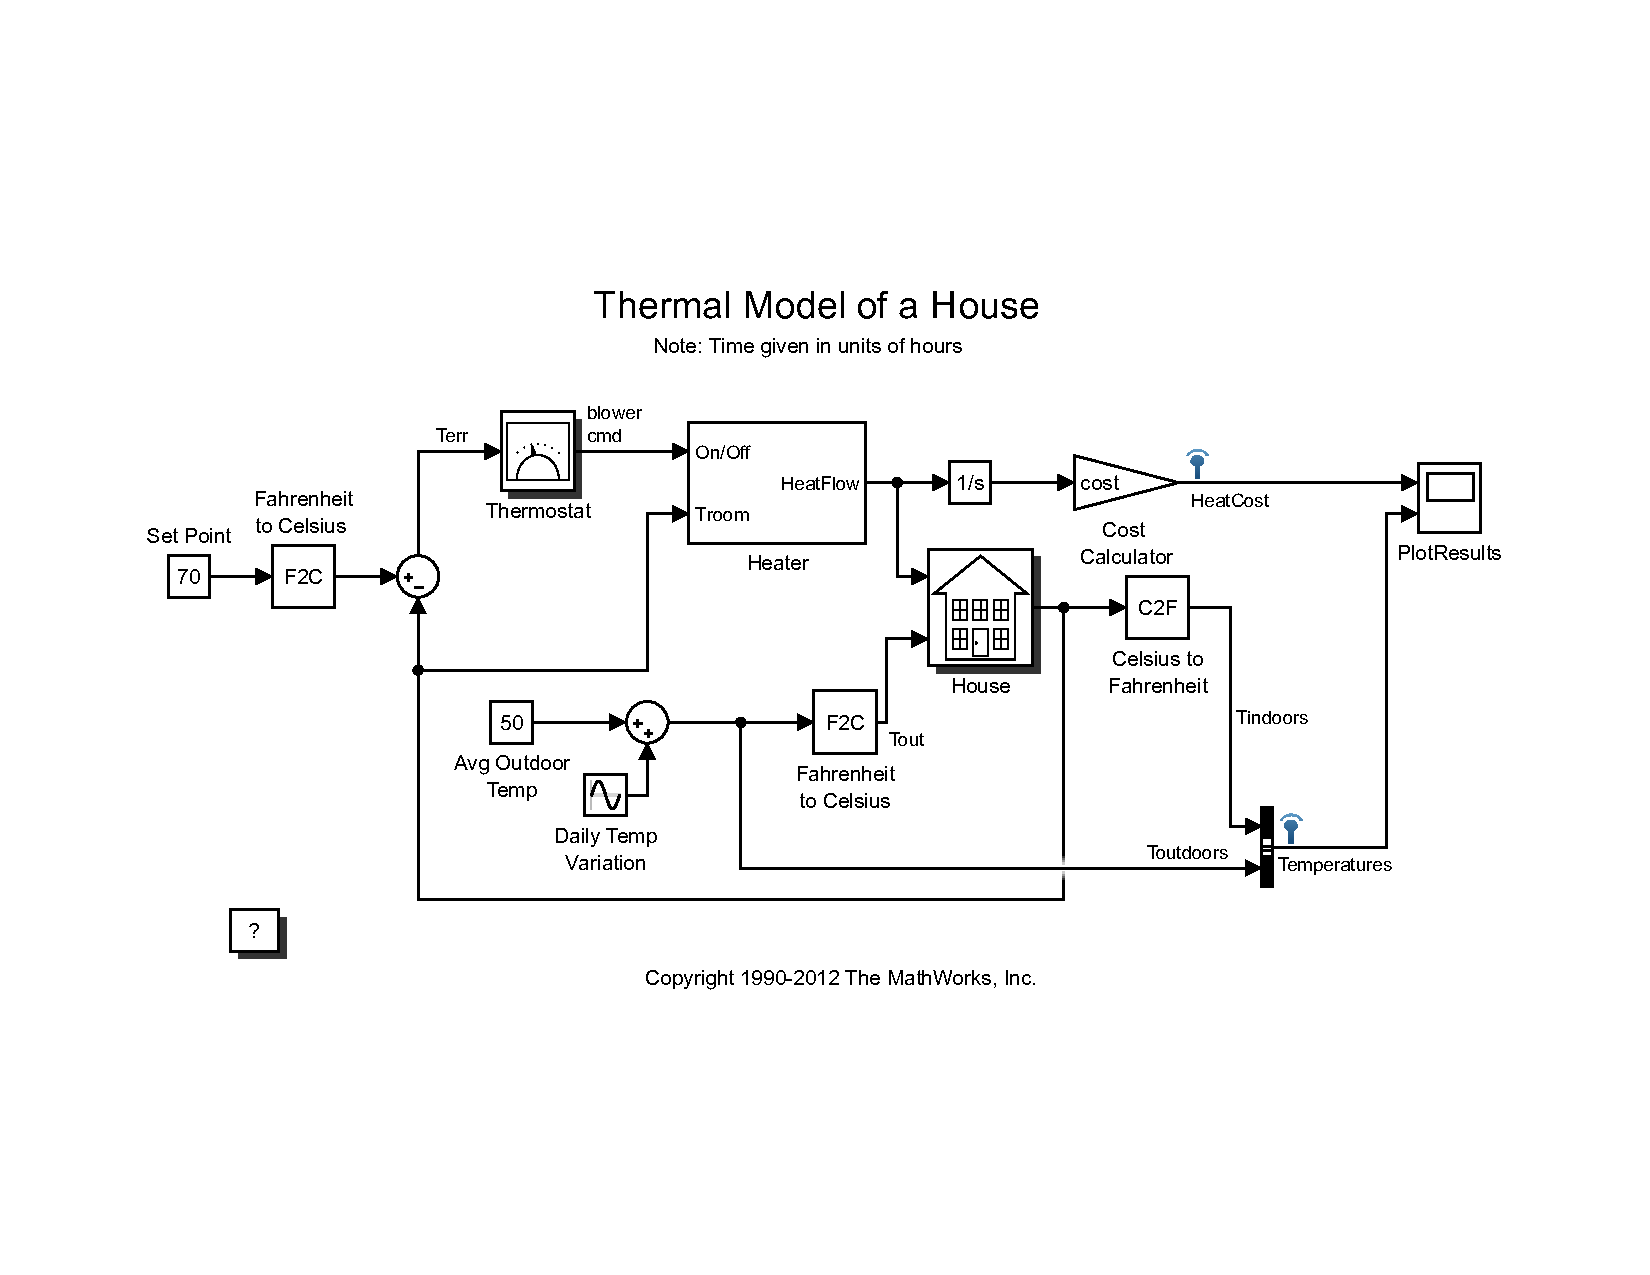
\includegraphics[trim={0 4.5cm 0 4.5cm},clip, width=\textwidth]{sldemo_househeat.pdf}}\\
\end{figure}

Open the model that contains the \topsystem{} by entering the following command in the \matlab{} command window:\\
\mcode{open\_system('PathToMyModel')}, replacing ``PathToMyModel'' with the full path of the model you copied earlier. 

%-------------------------------------------
\section*{Navigate to the desired save location}
\label{sec:Nav2DesSaveLoc}
%-------------------------------------------
The ``current folder'' in \matlab{} refers to the location where the generated \hyperref[acr:sdd]{SDD} document will be saved.
%, and can be identified and changed in several ways. 
Navigate to the desired folder e.g. with the address field, the current folder pane (shown in Figure \ref{fig:current-folder-1}), or the \mcode{cd} command\footnote{\href{https://www.mathworks.com/help/matlab/ref/cd.html}{https://www.mathworks.com/help/matlab/ref/cd.html}}.

\begin{figure}
	\caption{The current folder pane in \matlab{}. 
	Visual features may differ with current folder, settings, and \matlab{} version.}
	\centering
	\label{fig:current-folder-1}
	\fbox{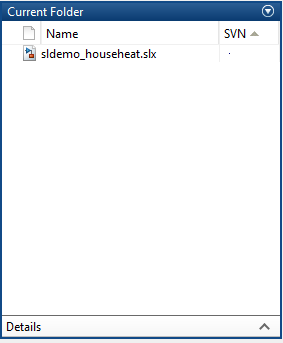
\includegraphics[scale=0.9]{PreGenCurrentFolder.PNG}}\\
\end{figure}

%-------------------------------------------
\section*{Generate the SDD document}
%-------------------------------------------
Next, we generate a preliminary \hyperref[acr:sdd]{SDD} document to view the document's structure before we start documenting our example. 
This step helps the user understand what else needs to be done to create the \hyperref[acr:sdd]{SDD} document, but is otherwise unnecessary. 
The \hyperref[acr:sdd]{SDD} document can be generated by clicking in the ``sldemo\_househeat'' \simulink{} system and then entering the following command in the \matlab{} command line: \mcode{GenSDD(gcs)}. 
Note that \mcode{gcs} points to the current \simulink{} system or the system which was most recently clicked in. 
Thus, we click in our \topsystem{},
(i.e., ``sldemo\_househeat'') first, and then enter the previous command in the \matlab{} command line. 
The \matlab{} command line window should look similar to the snapshot shown in Figure \ref{fig:gen-1} at the start of the \hyperref[acr:sdd]{SDD} document generation.

\begin{figure}
	\caption{A snapshot of the initial command window output after generating a	preliminary \hyperref[acr:sdd]{SDD} document for our example.}
	\centering
	\label{fig:gen-1}
	\fbox{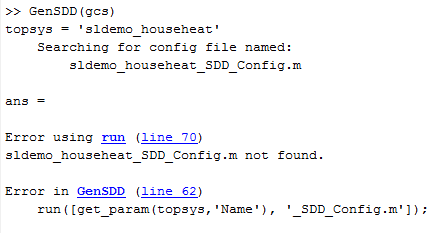
\includegraphics{Gen&MissingConfigFileError.PNG}}\\
\end{figure}

Additionally, a pop-up window similar to that shown in Figure \ref{fig:warning-pop-up} appears during the \hyperref[acr:sdd]{SDD} document generation to indicate
that there are warnings. 
The user should continue the \hyperref[acr:sdd]{SDD} document generation process, unless the user already knows what the warnings are for and how to fix them.

\begin{figure}
	\caption{A snapshot of the pop-up which appears during the \hyperref[acr:sdd]{SDD} document	generation if there were warnings.}
	\centering
	\label{fig:warning-pop-up}
	\fbox{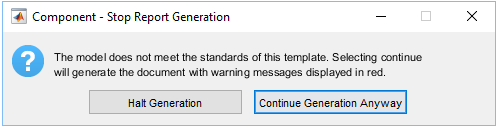
\includegraphics{WarningForWarningsPopUp.PNG}}\\
\end{figure}

Once generation has completed, two things occur. 
First, the generated files will appear in the current folder (as indicated by the \mcode{pwd} command). 
An updated view of the current folder pane should look similar to the snapshot shown in Figure \ref{fig:current-folder-2}. 
Second, the generated \hyperref[acr:sdd]{SDD} document should have opened automatically. 
If the warnings pop-up window shown in Figure \ref{fig:warning-pop-up} appeared to the user, then a ``Summary of Warnings'' chapter will be added at the bottom of the generated \hyperref[acr:sdd]{SDD} document. 
A snapshot of the chapter is shown in Figure \ref{fig:summary-of-warnings}. 
The ``Summary of Warnings'' chapter provides a list of the generated warnings, explaining their cause and solution.

% {\bf{G- note that i did get a popup, but the generated doc on my side had no
% chapter called ``Summary of warnings''. If that may be due to that I have an
% outdated version of the tool, thats ok. Otherwise, please fix the inconsistency
% between the doc and what the tool actually does.\\
% -GM:If it was the same pop-up as shown in the figure, then unfortunately I have
% no idea why that would happen off the top of my head, I might have to look at
% the example you tried in person or you could try describing it (I don't think
% there was ever a version in which it would not correspond to the creation of a
% Summary of Warnings section so hopefully I'm just forgetting something). I'm
% hesitant to make a change to what it says since I may have mentioned this in numerous other places as well.
% \\Update: (by the way, this is the potential bug I mentioned wanting to talk to
% you about).
% After more thought, this is probably because the example that you were referring
% to was outdated rather than because the tool was outdated. Was the warning in
% the Summary of Warnings about a missing Internal Design block?}} \\ {\bf{G-
% thats the thing, I didnt get a summary of warnings chapters in the first place
% so I cant answer ur question, but I did get the same exact popup msg\ldots NP,
% we'll comment this for now}}

% Since the purpose of this step is to experiment with the tool before adding any
% documentation to the \topsystem{}, %%The ``SDD\_sldemo\_househeat\_docx\_files''
% %%folder can now be deleted.
% the files you created so far in the Current Folder (that you specified in the 
% \hyperref[sec:Nav2DesSaveLoc]{``Navigate to the desired save location''}
% step) can now be deleted.
% {\bf{G- for the previous folder path, is that the full path?  Shouldnt there be
% a ``$\sim$/'' preceding it ? Besides, is this the only thing that should be
% deleted? shouldnt the user also delete the generated word document, since next
% theyll be generating an actual one with real documentation added ?\\
% -GM: It's not the full path, but if they are doing the example somewhere else on
% their machine it won't lead with ``$\sim$/\ldots''. It should correspond with
% the folder they went to in the ``Navigate to the desired save location'' section.\\
% As for file deletion, the original wording appears to have been that the folder
% ``may be'' deleted rather than ``can now be deleted'', this is because the
% folder may in general be deleted with no harm, but there is never any need to
% delete it; deleting it at this stage is fine as well though it's actually
% redundant since it will be generated again. I didnt mention the word document
% here because it would be redundant to delete it now since it will automatically
% be overwritten later anyway and later it should not be deleted.\\
% I did not make any edits here because I didn't want to go in circles by
% returning it to what I had, but it should be changed to reflect that the folder
% can be deleted freely at any point.}}

\begin{figure}
	\caption{An updated snapshot of the ``Current Folder'' pane after \hyperref[acr:sdd]{SDD} document generation.}
	\centering
	\label{fig:current-folder-2}
	\fbox{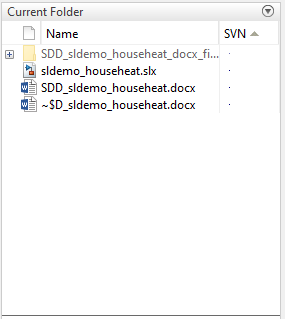
\includegraphics{PostGenCurrentFolder.PNG}}\\
\end{figure}
\begin{figure}
	\caption{A snapshot of the ``Summary of Warnings'' chapter in the generated	\hyperref[acr:sdd]{SDD} document.}
	\centering
	\label{fig:summary-of-warnings}
    \fbox{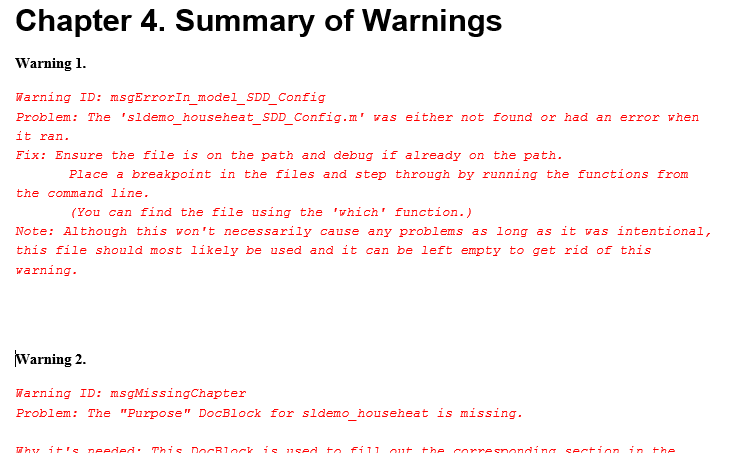
\includegraphics[width=\textwidth]{SummaryOfWarnings1.PNG}}\\
\end{figure}

%-------------------------------------------
\section*{Preparing the Configuration File}
%-------------------------------------------
The first warning shown in Figure \ref{fig:summary-of-warnings} indicates that the first thing to be done is to create the ``sldemo\_househeat\_SDD\_Config.m'' file. 
A template for this file can be found at: $\sim$/Report\_Specific\_Files/TopsysName\_SDD\_Config.m.

Copy this file to the location of your choosing on the search path and rename it to 
``sldemo\_househeat\_SDD\_Config.m''. 
% {\bf{G- hasnt this file already been
% copied and customized in the examples folder of your tool's folder? ie, the
% downloaded tool already has that file copied into the examples folder,
% correct? if yes, please reply to this comment and I'll update the text such
% that the user knows that this step has already been done, so that they wont
% create duplicate config file in the same folder\ldots \\
% -GM: I want to tell them how to get the stuff that is in the examples folder. So
% yes it is copied and customized in the examples folder but it's not copied and
% customized wherever they have their copy.}} 

As shown in Figure \ref{fig:folder-with-model-1}, we copied the file to the same folder containing the generated \hyperref[acr:sdd]{SDD} document and the sldemo\_househeat model that is used for this example.

\begin{figure}
	\caption{A snapshot showing the files in the folder where the \hyperref[acr:sdd]{SDD} document is saved. 
	These files need not be saved together.}
	\centering
	\label{fig:folder-with-model-1}
	\fbox{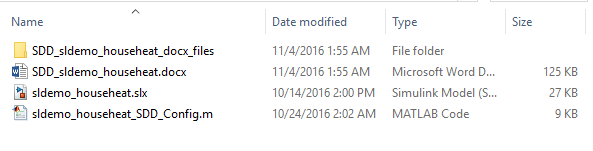
\includegraphics[width=\textwidth]{FolderWithModel1.PNG}}\\
\end{figure}

\newpage
Now, the config file needs to be modified. 
So, open the \\
``sldemo\_househeat\_SDD\_Config.m'' file. 
Figure \ref{fig:config-1} shows a snapshot of the file's contents.

\begin{figure}
	\caption{A snapshot of the initial configuration file.}
	\centering
	\label{fig:config-1}
	\fbox{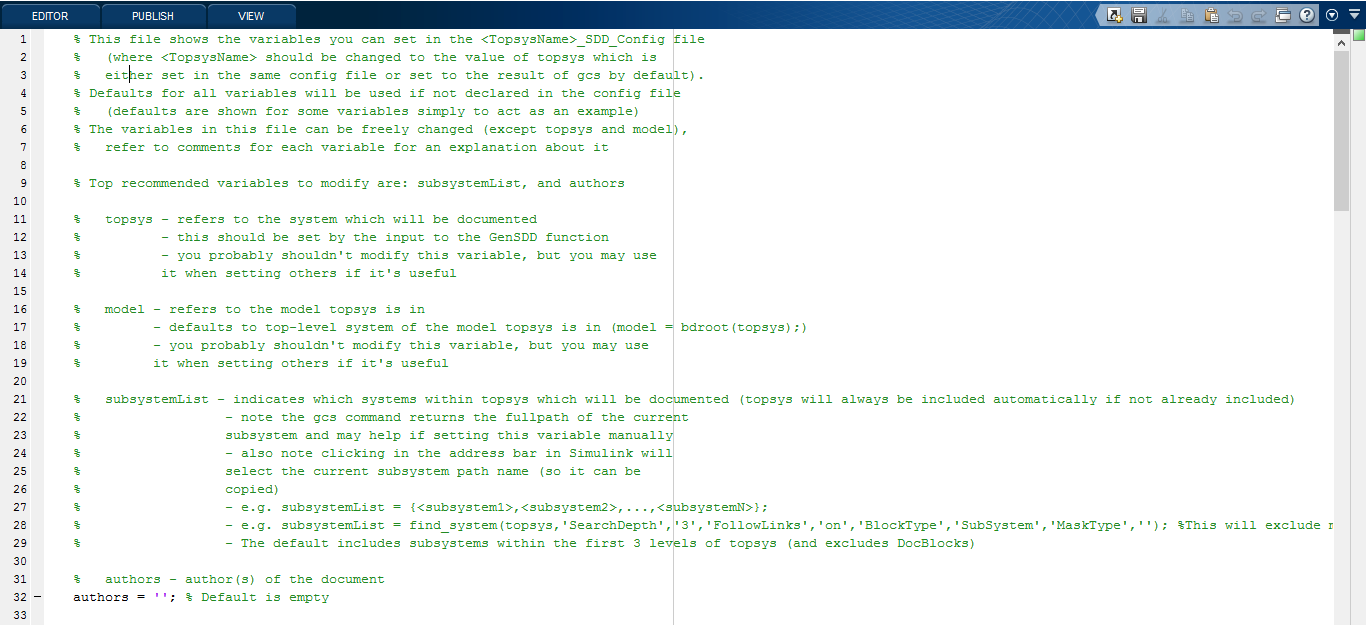
\includegraphics[width=\textwidth]{Config1.PNG}}\\
\end{figure}

This file is heavily commented and explains how to modify the different configuration parameters in detail. 
For this example, we will modify the $subsystemList$ variable and the $authors$ variable. The $subsystemList$ variable is the most important variable to set in this file. 
For the $subsystemList$ variable, we need to decide which subsystems to document within the \topsystem{}, and these systems will be referred to as the \sigsubs{}. 
For example, the user might just want to document the ``House'' subsystem in the \topsystem{}. 
The name that needs to be used for the $subsystemList$ variable is its fullname: ``sldemo\_househeat/House systems'' rather than just ``House''. 
To get the fullname of a system you can navigate to that system within \simulink{} and use either the \mcode{gcs} command or copy it from the address bar in \simulink{}. 
Figure \ref{fig:current-system-name} shows these two methods for the House subsystem.

\begin{figure}
    \centering
    \begin{subfigure}[c]{0.45\textwidth}
        \fbox{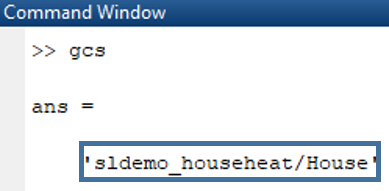
\includegraphics[width=\textwidth]{GetCurrentSystemName_CommandLine.PNG}}
        \caption{Retrieve the system's name using the \mcode{gcs} command.}
        \label{fig:gcs}
    \end{subfigure}
    ~
    \begin{subfigure}[c]{0.45\textwidth}
        \fbox{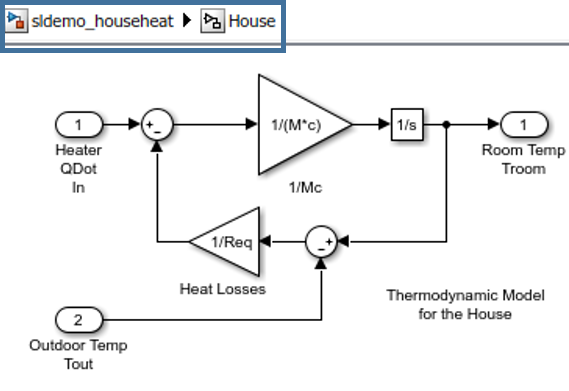
\includegraphics[width=\textwidth]{GetCurrentSystemName_AddressBar.PNG}}
        \caption{Retrieve the system's name from the \simulink{} address bar.}
        \label{fig:gcs-address-bar}
    \end{subfigure}
    \caption{Two ways to get the current system name.}\label{fig:current-system-name}
\end{figure}

Knowing the names of the \sigsubs{} and the author(s), the $subsystemList$ and the $authors$ variables can now be set as shown in Figure \ref{fig:config-2}.
%with the following two lines:
% \begin{itemize}
% 	\item[] \mcode{subsystemList = \{'sldemo\_househeat/House'\};}
% 	\item[] \mcode{authors = 'FirstName LastName';}
% \end{itemize}

\begin{figure}
	\caption{Setting the $subsystemList$ and the $authors$ variables for our example.}
	\centering
	\label{fig:config-2}
	\fbox{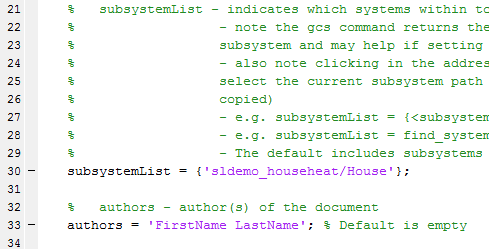
\includegraphics[width=\textwidth]{Config2.PNG}}\\
\end{figure}

Although the $subsystemList$ variable only includes one subsystem, the sldemo\_househeat system will be documented by default. 
For more complex
systems, the user might find it useful to add more subsystems to the $subsystemList$ variable.

To see how the document has changed, generate the \hyperref[acr:sdd]{SDD} document again. 
The command window output should look similar to the snapshot shown in Figure \ref{fig:gen-2}. 
The notable difference is that the errors that appeared in Figure \ref{fig:gen-1}, are now absent.

\begin{figure}
	\caption{A snapshot of the initial command window output for the second \hyperref[acr:sdd]{SDD}	document generation in this example, and the warning pop-up.}
	\centering
	\label{fig:gen-2}
	\fbox{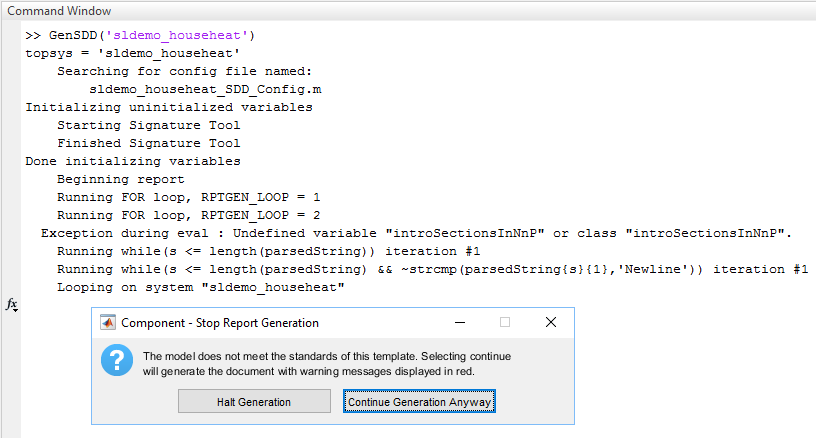
\includegraphics[width=\textwidth]{Gen2&WarningForWarningsPopUp2.PNG}}\\
\end{figure}

Looking at the first page of the generated \hyperref[acr:sdd]{SDD} document (shown in Figure \ref{fig:title-page-2}), one can see that the author indicated in the
configuration file will now appear here.

\begin{figure}
	\caption{A snapshot of the title page for the example with the author(s) set to	`FirstName LastName'.}
	\centering
	\label{fig:title-page-2}
	\fbox{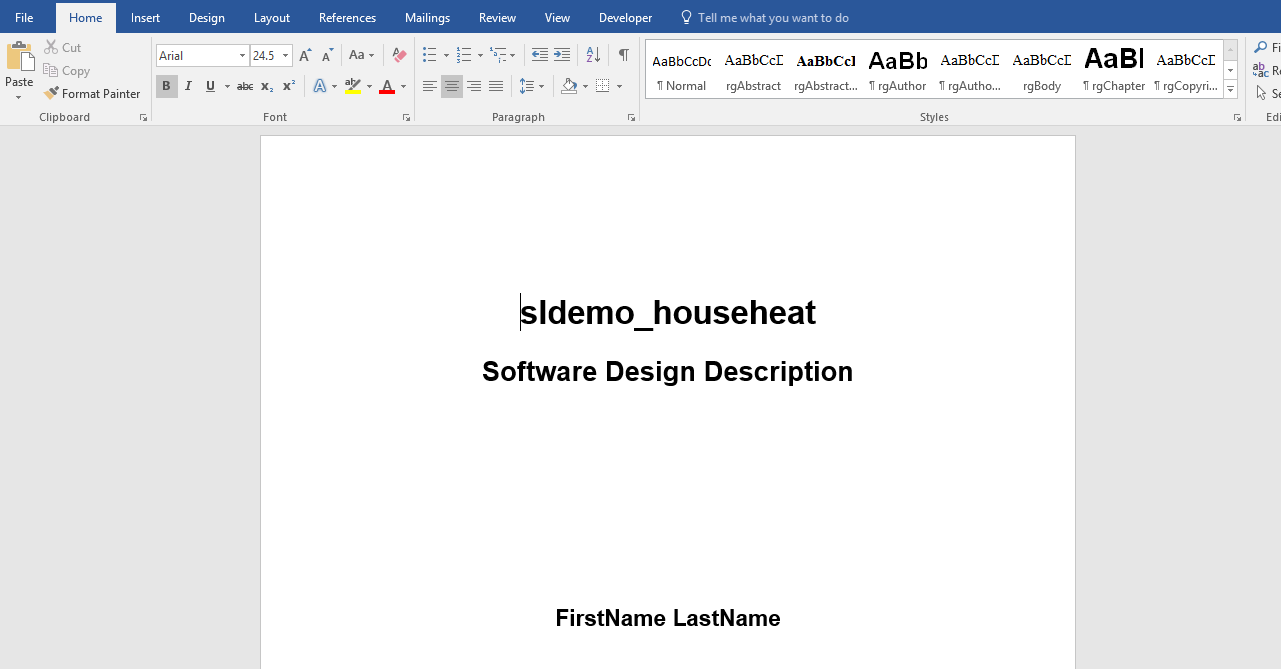
\includegraphics[width=\textwidth]{TitlePage2.PNG}}\\
\end{figure}

Another notable change is in the structure of the overall \hyperref[acr:sdd]{SDD} document. 
Previously, it had been set up by default to describe more systems. 
Currently, given that the $subsystemList$ variable has been set, the structure was changed to only provide sections for the sldemo\_househeat and the sldemo\_househeat/House systems. 
Figure \ref{fig:toc-2} shows the Table of Contents of the newly generated \hyperref[acr:sdd]{SDD} document.

\begin{figure}
	\caption{A snapshot of the table of contents of the updated \hyperref[acr:sdd]{SDD} document.}
	\centering
	\label{fig:toc-2}
	\fbox{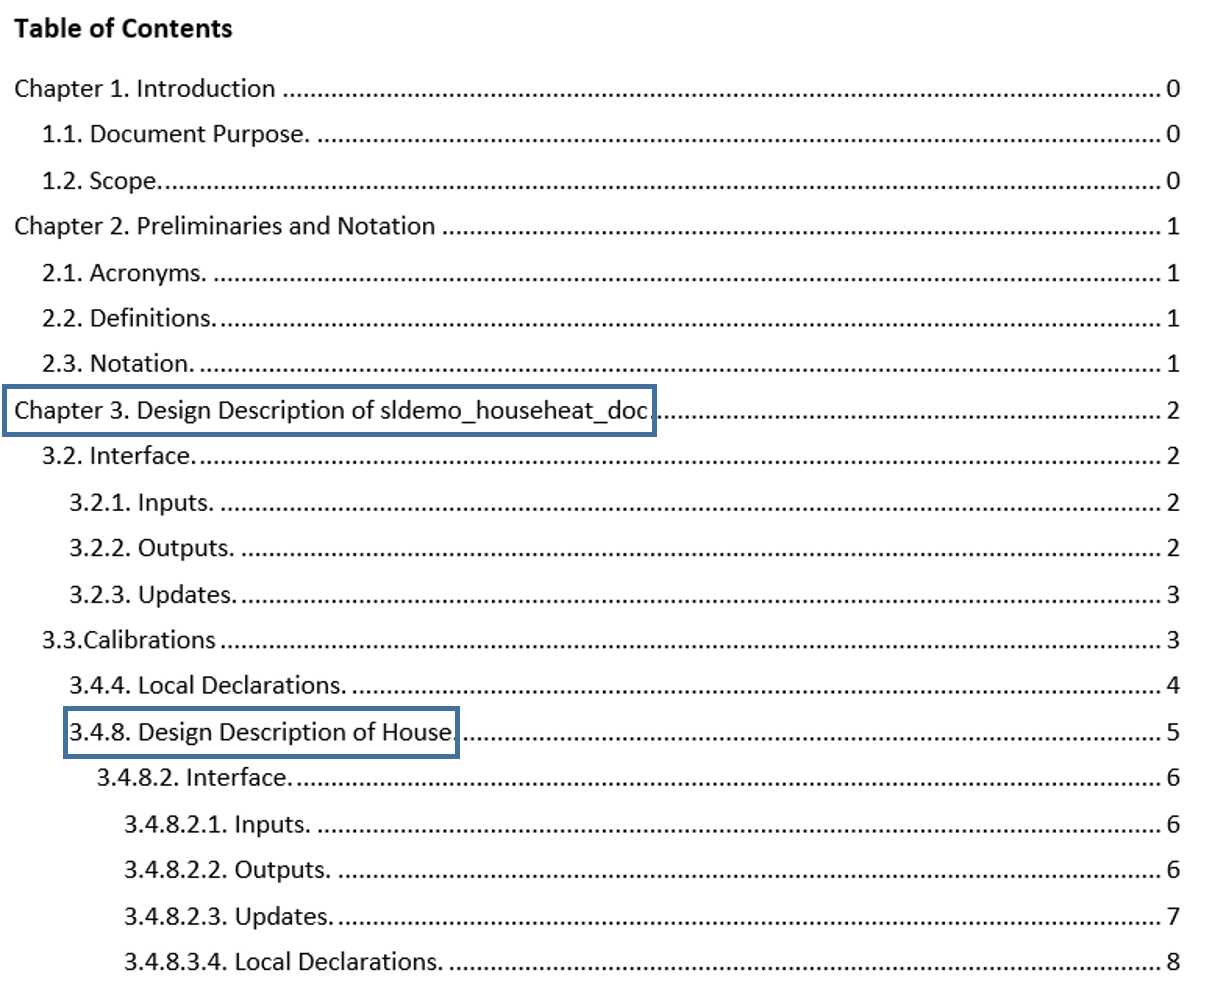
\includegraphics[width=\textwidth]{ToC2.PNG}}\\
\end{figure}

%-------------------------------------------
\section*{Adding the Required Documentation}
%-------------------------------------------
The ``Summary of Warnings'' chapter in the generated \hyperref[acr:sdd]{SDD} document shows which warnings need to be addressed, and hence what additional steps need to be done to generate an informative \hyperref[acr:sdd]{SDD} document. 
Figure \ref{fig:summary-of-warnings-2} shows some of these warnings.

\begin{figure}
	\caption{A snapshot of the ``Summary of Warnings'' chapter after the second \hyperref[acr:sdd]{SDD}	document generation.}
	\centering
	\label{fig:summary-of-warnings-2}
	\fbox{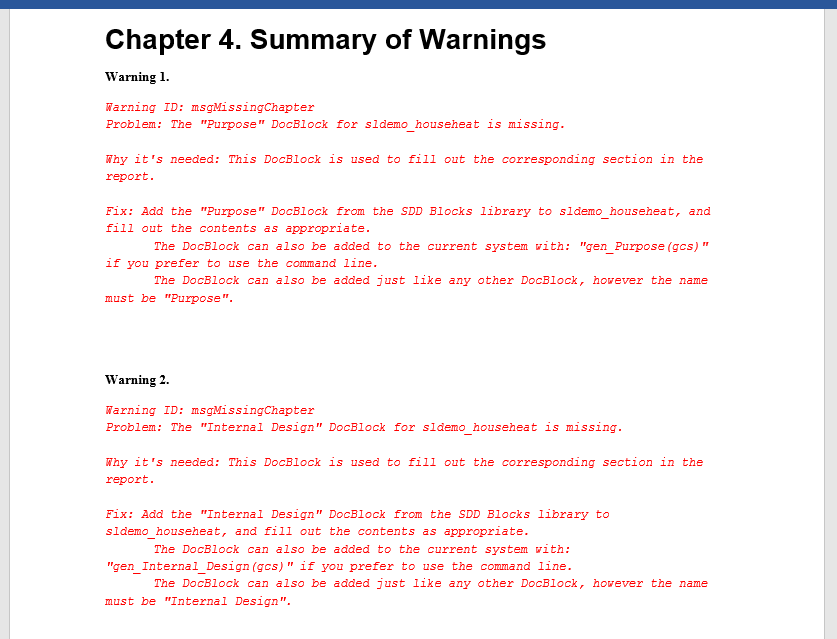
\includegraphics[width=\textwidth]{SummaryOfWarnings2.PNG}}\\
\end{figure}

At this point, eight warnings remain, all of which share the same Warning ID, i.e., they all describe a similar problem with a similar fix.
The following steps will be performed to fix each of these warnings.

First, open the Library Browser e.g. using the \mcode{slLibraryBrowser} command or by clicking the appropriate button from \simulink{}, as shown in Figure \ref{fig:open-lib-browser}. 
Note that the aforementioned button shown in Figure~\ref{fig:open-lib-browser}
may differ between \matlab{} versions.

\begin{figure}
	\caption{A snapshot demonstrating the button to click to open the Library Browser.}
	\centering
	\label{fig:open-lib-browser}
	\fbox{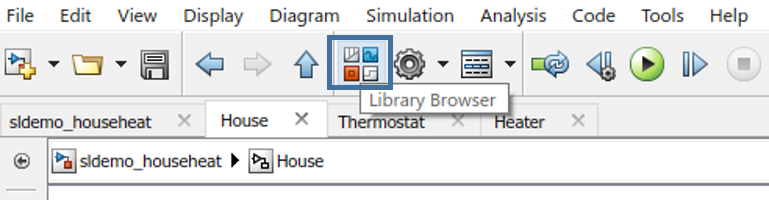
\includegraphics{OpenLibraryBrowser.png}}\\
\end{figure}

After the Library Browser opens, navigate in the left pane to SDD Blocks. 
Three sets of blocks appear, two of which provide optional blocks and one provides blocks which are required to appropriately document the system. 
For this example, we are interested in the latter option which is labeled ``Required SDD\_Blocks For Documented (Sub)Systems''. 
Figure \ref{fig:lib-browser} shows where the desired option is within the Library Browser. 
By analyzing the warnings in the generated \hyperref[acr:sdd]{SDD} document, one can notice that the warnings stated that one of these blocks was missing from either the sldemo\_househeat system or the sldemo\_househeat/House system. 
Thus, our goal is to drag and drop these blocks within those systems. 
Figures \ref{fig:ex-topsys-2} and \ref{fig:house-2} show the sldemo\_househeat and the sldemo\_househeat/House systems after adding the blocks grouped in the ``Required SDD\_Blocks For Documented (Sub)Systems'' to them.

\begin{figure}
	\caption{A snapshot of the Library Browser, showing the required blocks	for generating \hyperref[acr:sdd]{SDD} documents using our tool.}
	\centering
	\label{fig:lib-browser}
	\fbox{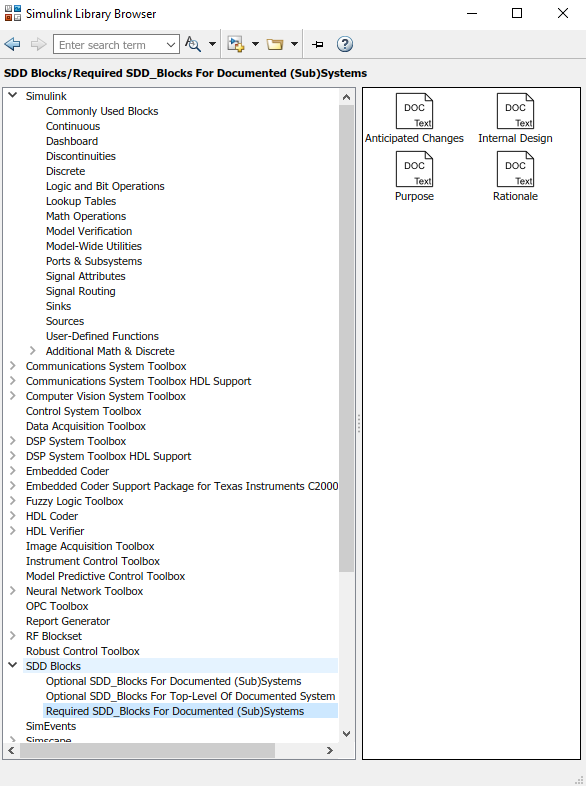
\includegraphics[width=\textwidth]{LibraryBrowser.PNG}}\\
\end{figure}
\begin{figure}
	\caption{A snapshot of the sldemo\_househeat system after adding the required	\textsf{DocBlocks} to it.}
	\centering
	\label{fig:ex-topsys-2}
	\fbox{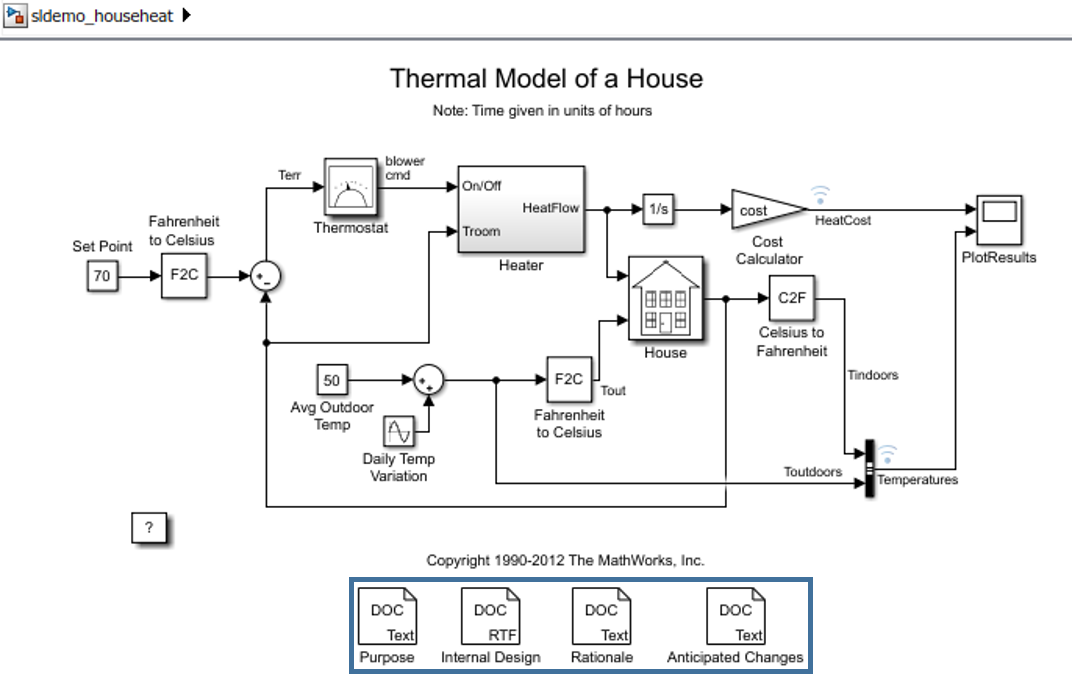
\includegraphics[width=\textwidth]{sldemo_househeat2.png}}\\
\end{figure}
\begin{figure}
	\caption{A snapshot of the House system after adding the required \textsf{DocBlocks} to it.}
	\centering
	\label{fig:house-2}
	\fbox{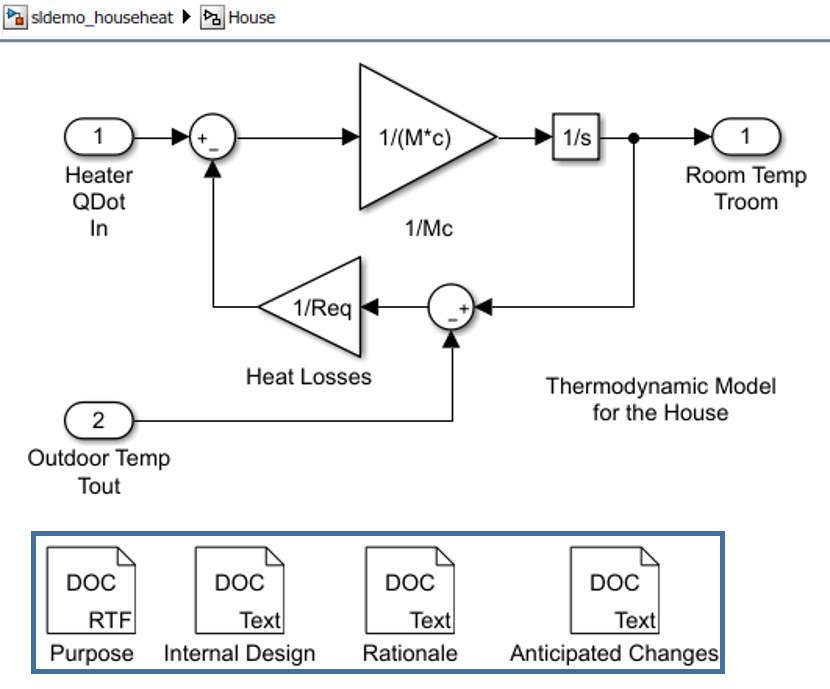
\includegraphics[scale=0.8]{House2}}\\
\end{figure}

The \hyperref[acr:sdd]{SDD} document can now be regenerated since the warnings were addressed. 
However, new warnings will be produced, as shown in Figure~\ref{fig:summary-of-warnings-3}.

\begin{figure}
	\caption{A snapshot of the Summary of Warnings chapter after the third attempt at generating the \hyperref[acr:sdd]{SDD} document for our example.}
	\centering
	\label{fig:summary-of-warnings-3}
	\fbox{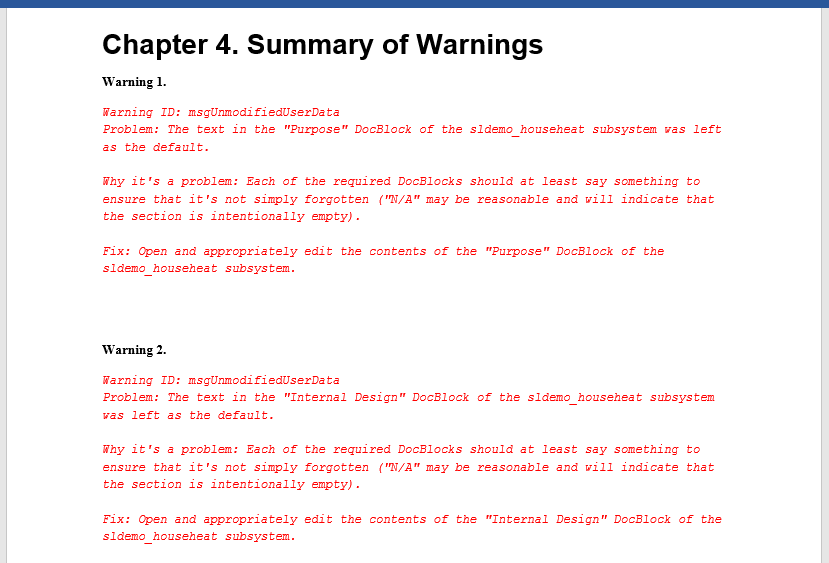
\includegraphics[width=\textwidth]{SummaryOfWarnings3.PNG}}\\
\end{figure}

These warnings indicate that there is unmodified data in the blocks that were added. 
Such warnings are due to the fact that the \sddtool{} checks to ensure
that the user does not simply add these blocks without modifying their contents. 
Thus, to address these warnings, the user should modify the contents of the blocks by double-clicking the blocks and adding the necessary documentation to each block. 
For example, double-clicking the Purpose block from the sldemo\_househeat system will open its contents to reveal text as shown in Figure~\ref{fig:purpose-1}.

\begin{figure}
	\caption{A snapshot of the default contents of the Purpose blocks from the SDD Blocks library.}
	\centering
	\label{fig:purpose-1}
	\fbox{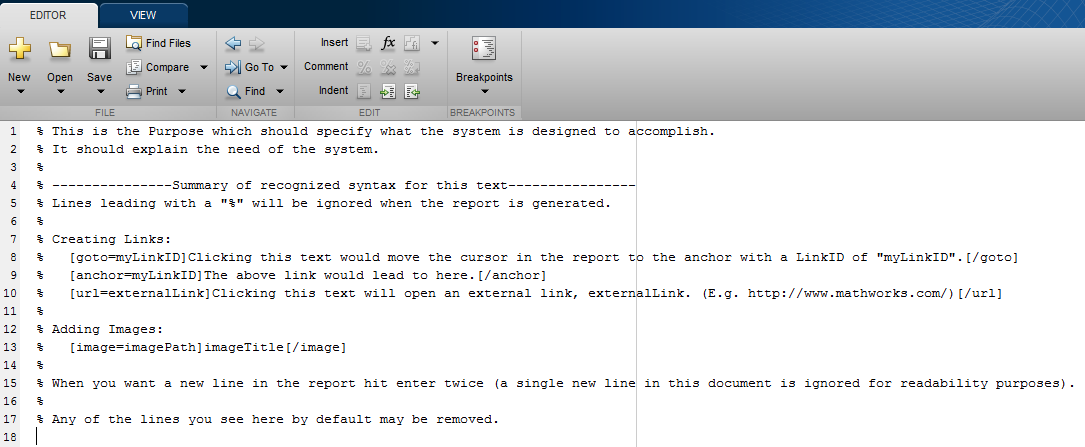
\includegraphics[width=\textwidth]{PurposeDocBlock1.PNG}}\\
\end{figure}

Note that the default text in the \sddblks{} blocks consists of a number of lines preceded by a percent symbol, `\%'. 
These lines are comments and thus, will not be included in the generated \hyperref[acr:sdd]{SDD} document. 
These comments describe some features that are accessible through the text in
the \sddblks{} blocks.

As for what to add in the \sddblks{} blocks, the user should add any necessary information that they believe will sufficiently describe how the system works. 
The amount of information to add varies between systems, depending on their complexity. 
For the purpose of our example, we add text to the blocks based on information found on \mathworks{} page about the sldemo\_househeat model\footnote{\href{http://www.mathworks.com/help/simulink/examples/thermal-model-of-a-house.html}{www.mathworks.com/help/simulink/examples/thermal-model-of-a-house.html}}. 
The text added to the Purpose block is shown in Figure~\ref{fig:purpose-2}. 
The user will notice that we have also created a link to \mathworks{} page about the sldemo\_househeat model within this block's text using tags defined in the comments. 
This file needs to be saved before closing it, for the block to be changed within the model. 
Saving this file will not save the model. 
Do not be concerned with the save location or what it is saved as, simply press \mcode{ctrl+S} before closing the file.

\begin{figure}
	\caption{A snapshot of the Purpose block after adding a short description of the system from The Mathworks.}
	\centering
	\label{fig:purpose-2}
	\fbox{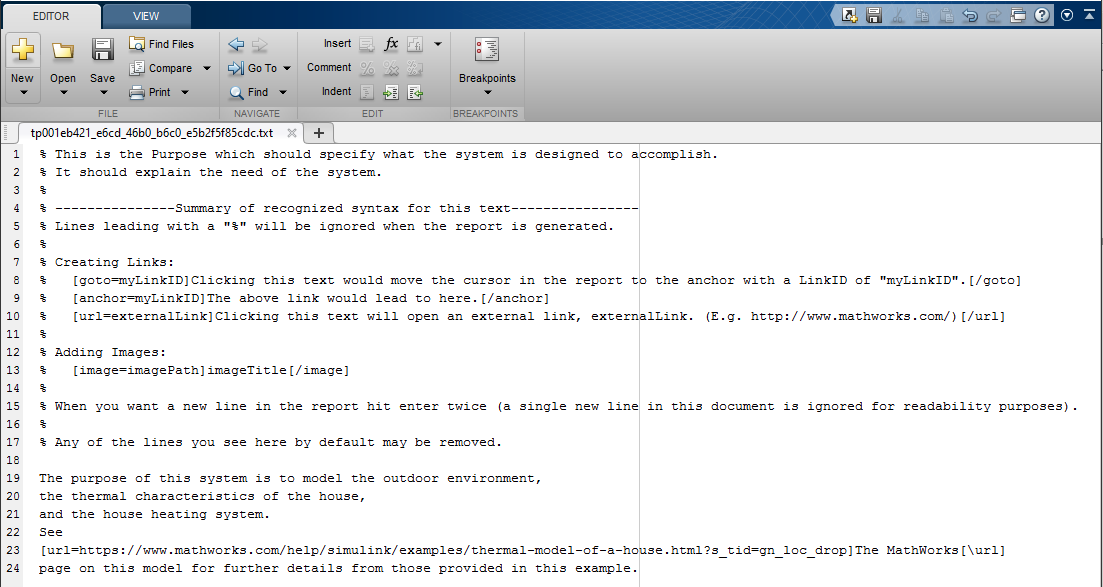
\includegraphics[width=\textwidth]{PurposeDocBlock2.PNG}}\\
\end{figure}

If the text interface shown in Figure~\ref{fig:purpose-1} and Figure~\ref{fig:purpose-2} is not desired, note that a format more similar to Microsoft Word may also be used (either way the final generated document will be a Microsoft Word document). 
The blocks in the \sddblks{} are made from \textsf{DocBlocks}, which can be formatted in different ways. 
To change the format for the Internal Design block for example, right-click the Internal Design block and select ``Mask'' then ``Mask Parameters...'', as shown in Figure \ref{fig:open-mask-param}.

\begin{figure}
	\caption{A snapshot showing how to open the mask parameters of a block in	\matlab{} R2016b.}
	\centering
	\label{fig:open-mask-param}
	\fbox{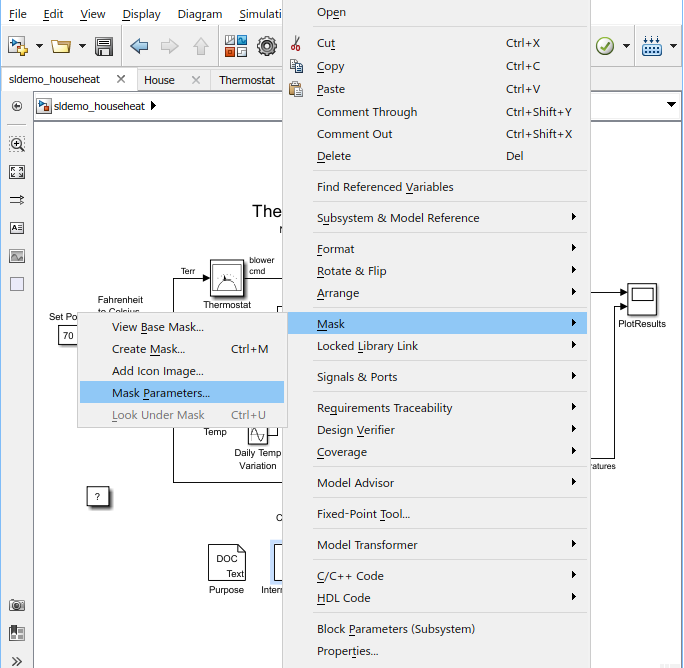
\includegraphics[width=\textwidth]{OpenMaskParameters.png}}\\
\end{figure}

From the window that opens, select ``RTF'' (Figure \ref{fig:mask-param}) from the drop down menu, then click ``Apply''. 
The image of the block in the system now says ``RTF'' in place of ``Text'', which was there previously. 
In general, DocBlocks in used with the \sddtool{} always use either the Text or RTF format (not HTML).

\begin{figure}
	\caption{A snapshot of the ``Block Parameters'' window showing the ``Document	type'' dropdown.}
	\centering
	\label{fig:mask-param}
	\fbox{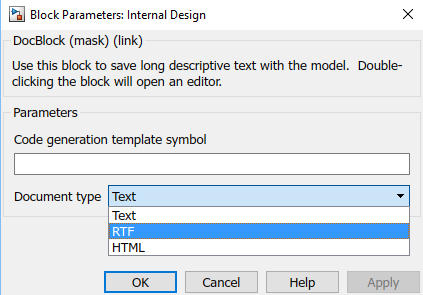
\includegraphics[scale=0.8]{MaskParameters.png}}\\
\end{figure}

Now double-click the Internal Design block to see its contents (shown in Figure~\ref{fig:int-des-rtf}).

\begin{figure}
	\caption{A snapshot of the default contents of an Internal Design block from the \sddblks{} if its format is changed to RTF.}
	\centering
	\label{fig:int-des-rtf}
	\fbox{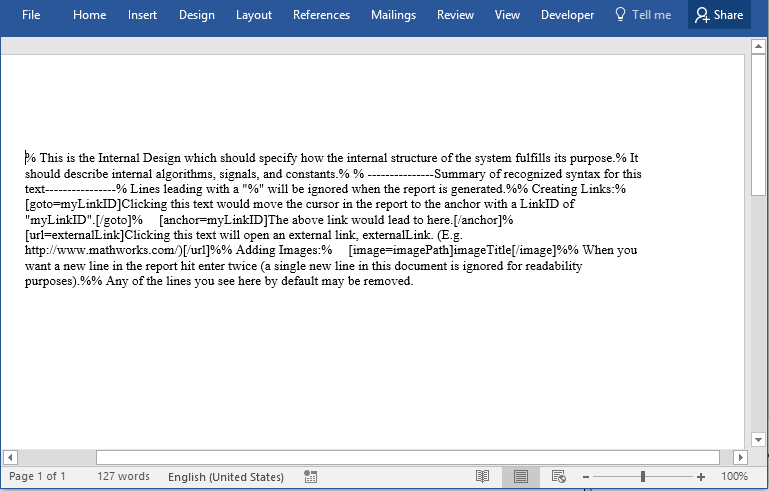
\includegraphics[width=\textwidth]{InternalDesignRTF.PNG}}\\
\end{figure}

The contents which the Internal Design block would have had in its Text format are now in this RTF file. 
However, unlike the text file, the percent symbol no longer indicates content to be ignored, i.e., any content in the RTF file will appear in the generated \hyperref[acr:sdd]{SDD} document. 
Additionally, any instructions following the ``Summary of recognized syntax for this text'' shown in Figure~\ref{fig:int-des-rtf}, no longer apply since that syntax is intended for text files. 
A description of the internal design can be added to the file, as shown in Figure~\ref{fig:int-des-rtf-2}.

\begin{figure}
	\caption{A snapshot of the Internal Design block after removing the default
	text and adding an appropriate description.}
	\centering
	\label{fig:int-des-rtf-2}
	\fbox{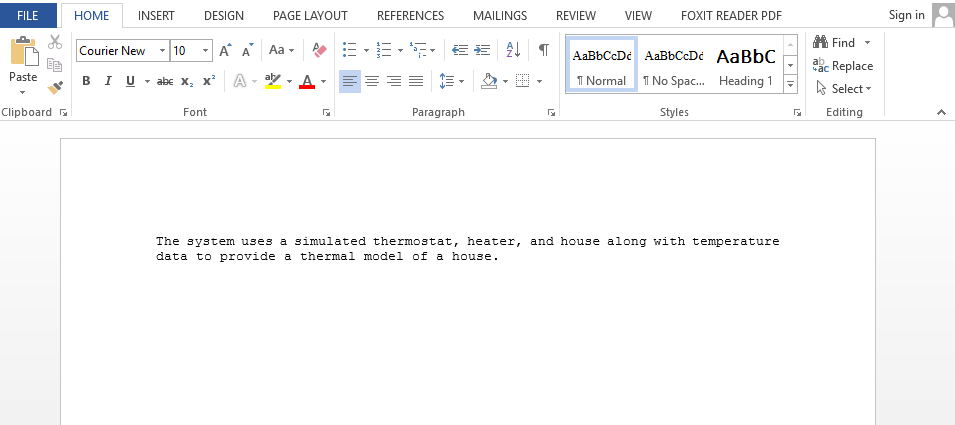
\includegraphics[width=\textwidth]{InternalDesignRTF2.PNG}}\\
\end{figure}

Save the contents of the file before closing. 
Now, continue to fill out the content of the remaining six blocks from the \sddblks{}. 
Figures~\ref{fig:househeat-sdd-blocks-2}~and~\ref{fig:House-sdd-blocks-2} show the remaining six \sddblks{} blocks we created for this example. 
Note that the Rationale blocks have no descriptive text since we were not the developers of this model and we could not find any documentation for it.

\begin{figure}
	\centering
	\caption{Contents of the Rationale and Anticipated Changes \sddblks{} blocks for the sldemo\_househeat system.}\label{fig:househeat-sdd-blocks-2}
	\begin{subfigure}[b]{\textwidth}
		\caption{Contents of the Rationale block for the sldemo\_househeat system.}
		\fbox{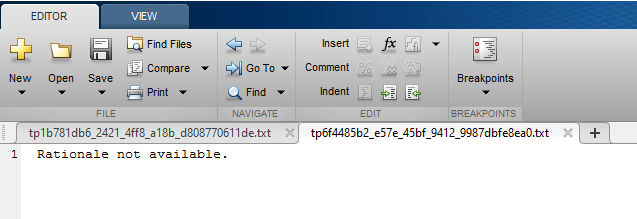
\includegraphics[width=\textwidth]{RationaleDocBlock2.PNG}}
		\label{fig:rationale-2}
	\end{subfigure}
	\begin{subfigure}[b]{\textwidth}
		\caption{Contents of the Anticipated Changes block for the sldemo\_househeat system.}
		\fbox{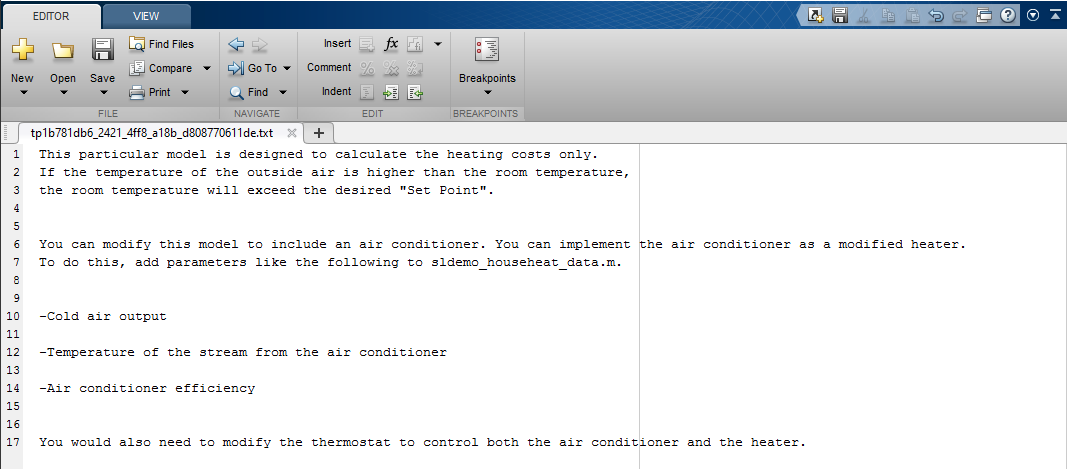
\includegraphics[width=\textwidth]{AntChangesDocBlock2.PNG}}
		\label{fig:ant-changes-2}
	\end{subfigure}
\end{figure}

\begin{figure}
	\centering
	\caption{Contents of all \sddblks{} blocks for the sldemo\_househeat/House	system.}
	\label{fig:House-sdd-blocks-2}
	\begin{subfigure}[t]{\textwidth}
		\caption{Contents of the Purpose block for the sldemo\_househeat/House system.}
		\fbox{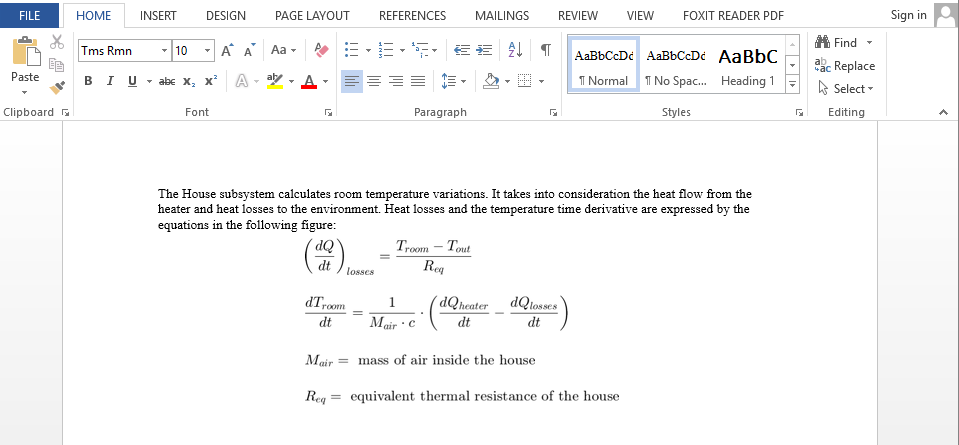
\includegraphics[width=\textwidth]{HousePurposeDocBlock2.PNG}}
		\label{fig:house-purpose-2}
	\end{subfigure}
	\begin{subfigure}[t]{\textwidth}
		\caption{Contents of the Internal Design block for the sldemo\_househeat/House system.}
		\fbox{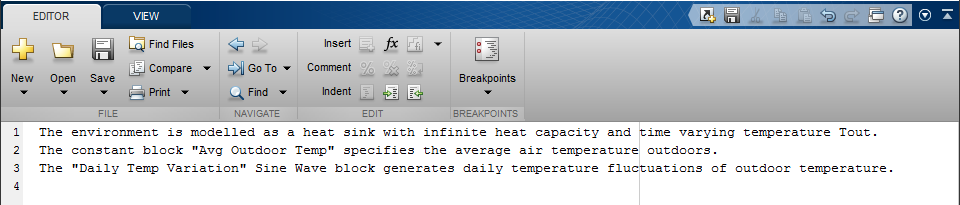
\includegraphics[width=\textwidth]{HouseInternalDesignDocBlock2.PNG}}
		\label{fig:house-int-des-2}
	\end{subfigure}
	\begin{subfigure}[t]{0.45\textwidth}
		\caption{Contents of the Rationale block for the sldemo\_househeat/House system.}
		\fbox{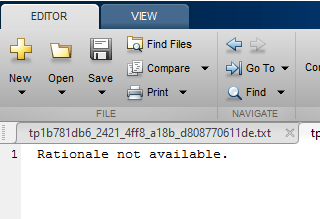
\includegraphics[width=\textwidth]{HouseRationaleDocBlock2.PNG}}
		\label{fig:house-rationale-2}
	\end{subfigure}
	~
	\begin{subfigure}[t]{0.45\textwidth}
		\caption{Contents of the Anticipated Changes block for the sldemo\_househeat/House system.}
		\fbox{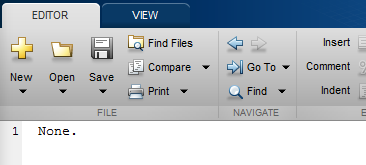
\includegraphics[width=\textwidth]{HouseAntChangesDocBlock2.PNG}}
		\label{fig:house-ant-changes-2}
	\end{subfigure}
\end{figure}

After adding documentation to all of the \sddblks{} blocks, the user can generate the \hyperref[acr:sdd]{SDD} document again. 
There should no longer be a pop-up window during the document generation, and the ``Summary of Warnings'' chapter should no longer appear in the \hyperref[acr:sdd]{SDD} document. 
This indicates that your \hyperref[acr:sdd]{SDD} document is complete and has all the required information! The document we generated at this stage can be viewed at:\\
``$\sim$/example/sldemo\_househeat\_doc/SDD\_sldemo\_househeat\_doc.docx''.

Chapter~\ref{ch:doc-process} of this user guide will describe in depth additional steps to prepare an \hyperref[acr:sdd]{SDD} document using our tool, and will explain other features that were not discussed in this chapter.

%====================================================================
\chapter{Structure of the Generated SDD Document}
\label{ch:sdd-output}
%====================================================================
This chapter describes the structure (and potential content) of the \hyperref[acr:sdd]{SDD} document generated by the \sddtool{}. 
Detailed steps describing how to generate this \hyperref[acr:sdd]{SDD} document are discussed in Chapter~\ref{ch:doc-process}.

To facilitate understanding the structure of the generated \hyperref[acr:sdd]{SDD} document, section names in this chapter closely correspond to section names in the generated \hyperref[acr:sdd]{SDD} document, and have the same order as in the generated SDD document.

%-------------------------------------------
\section{Title Page} 
\label{sec:title-page}
%-------------------------------------------
The generated \hyperref[acr:sdd]{SDD} document starts with a title page, that includes the document's title, subtitle, list of authors, and possibly an image (e.g. the logo of the company that generated the \hyperref[acr:sdd]{SDD} document).

%-------------------------------------------
\section{Copyright/Abstract/Legal Notice}
%-------------------------------------------
This section provides some information about the document and a copyright notice, and may include abstract and legal notice.

%-------------------------------------------
\section{Changelog}
\label{sec:changelog}
%-------------------------------------------
The Changelog section contains a table of the changes made to the system over time. 
For every change, the table includes the date of the change, the version of the file, a description of the changes made, the sections affected by the changes made, and the author of the changes.

%-------------------------------------------
\section{Table of Contents}
\label{sec:toc}
%-------------------------------------------
The Table of Contents contains a numbered list of the sections in the \hyperref[acr:sdd]{SDD} document and their page numbers. 
Each section in the Table of Contents acts as a link that can be used to navigate to the corresponding section.

%-------------------------------------------
\section{Introduction}
\label{sec:intro-description}
%-------------------------------------------
This section introduces readers to \hyperref[acr:sdd]{SDD} documents in general, and is not specific to the documented \topsystem{}. 
This section has two subsections: Document Purpose and Scope.
  
	\subsection{Document Purpose}
	\label{ssec:doc-purpose-description}
	This section explains the purpose of the \hyperref[acr:sdd]{SDD} document.
    
	\subsection{Scope}
	\label{ssec:scope-description}
	This section elaborates on what should and should not be included in the generated \hyperref[acr:sdd]{SDD} document. 

%-------------------------------------------       
\section{\gloss{}}
\label{sec:not-and-prelim}
%-------------------------------------------
The \gloss{} of the generated \hyperref[acr:sdd]{SDD} document contains acronyms, definitions, and notations that may help the reader understand the \hyperref[acr:sdd]{SDD} document.
  
\subsection{Acronyms} \label{ssec:acr-description}

\paragraph*{General Acronyms}
\label{par:acr-gen-description}
This list explains any acronyms that will be useful for the reader of the \hyperref[acr:sdd]{SDD} document. 
For example, it may include acronyms commonly used in industry.
      
\paragraph*{System Specific Acronyms}
\label{par:acr-sys-spec-description}
This list\label{itm:sys-acrs} explains acronyms specifically relevant to the \topsystem{}, that users of the \topsystem{} may not be aware of.

\subsection{Definitions}
\label{ssec:def-description}

\paragraph*{General Definitions}
\label{par:def-gen-description}
This list explains definitions that will be useful for the reader of the \hyperref[acr:sdd]{SDD} document. 
For example, it may include jargon commonly used in industry.

\paragraph*{System Specific Definitions}
\label{par:def-sys-spec-description}
This list\label{itm:sys-defs} explains definitions specifically relevant to the \topsystem{}, that users of the \topsystem{} may not be aware of.

\subsection{Notation}
\label{ssec:not-description}

\paragraph*{General Notation}
\label{par:not-gen-description}
This list explains notations that will be useful for the reader of the \hyperref[acr:sdd]{SDD} document. 
For example, it may include an explanation of the naming conventions used in the organization for which the \hyperref[acr:sdd]{SDD} document is generated, or it may describe a graphical notation commonly used within the organization.

\paragraph*{System Specific Notation} \label{par:not-sys-spec-description}
This list\label{itm:sys-not} explains notations that will be used in the \hyperref[acr:sdd]{SDD} document of the \topsystem{}. 
This may include an explanation of naming conventions used in the \topsystem{} or it may refer to a graphical notation used in a diagram in the \hyperref[acr:sdd]{SDD} document. 

%-------------------------------------------
\section{Design Description} 
\label{sec:des-desc}
%-------------------------------------------
The Design Description section comprises the bulk of the \hyperref[acr:sdd]{SDD} document and explains how the \topsystem{} works through its many subsections. 
This section sufficiently describes the inner workings of the \topsystem{} such that any user who is unfamiliar with it can easily figure out how it works, and understand how to modify the \topsystem{} to implement new features or to address issues.

%TODO cite the SEforDE paper - I'm not really sure how I should cite it
% specifically, I referred to it for purpose, internal design, rationale, and
% anticipated changes. Should it just be a citation at the bottom of the guide
% since I don't directly quote it?
  
    \subsection{Purpose} \label{ssec:purpose-description}
    This section describes \emph{what} the given system is designed to accomplish, i.e., the function of the system. 
    %\textbf{GM: changed from the
    % need for the system -since need implied why rather than what} % with respect to the \topsystem{}.
	  %  	  Report: The Purpose should provide a description of what the system is designed to accomplish.
    %  	  From SEforDE: ...a clear statement describing what the system is ultimately meant to accomplish.
    %  	  It is meant to reinforce the understanding of why the system needs to be developed.

    \subsection{Interface} 
    \label{ssec:interface-description}
    
In the context of \simulink{}, a system's interface is the set of blocks that act as either input or output to that system. 
While it is not difficult in \simulink{} to see that inports and outports act as inputs and outputs to systems, these are not the only blocks that can impact the system's functionality. 
Other blocks that can be in an interface include data store blocks and goto/from blocks. 
These blocks are capable of passing data into or out of a system without the need of a signal line connection.

The Interface section in the generated \hyperref[acr:sdd]{SDD} document has four subsections, namely \emph{Inputs}, \emph{Outputs}, and \emph{Updates}. 
The Inputs
subsection displays information on inports, data store reads, global froms, and scoped froms. 
The Outputs subsection displays information on outports, data store writes, global gotos, and scoped gotos. 
The Updates subsection will give different results depending on how the \sigtool{} is called. 
If the \sigtool{} is called in the default manner, then the Updates section will list data stores and goto tags that are both read from and written to. 

Each of the three aforementioned subsections displays the blocks in the given system's interface in tables. 
The specifics about the blocks that go in each table are determined by the \sigtool{}. 
Information given for each block includes:\\
    \begin{description}
      \item [Name\label{itm:int-name-description}] An identifier for the block that is unique within a system.
      \item [Units\label{itm:int-units-description}] E.g., $m$, $m/s^2$, $N*m$.
      \item [Min\label{itm:int-min-description}] The lower bound on the block's output value.
      \item [Max\label{itm:int-max-description}] The upper bound on the block's output value.
      \item [Data type\label{itm:int-datatype-description}] E.g., double, int8, boolean.
      \item [Description\label{itm:int-descr-description}] A description of the block.
    \end{description}
    
    \subsection{Calibrations}
    \label{ssec:calibrations}
    The calibrations section is only included if the given system is the \topsystem{}. 
    If applicable, it includes tables listing configurable constants (or variables) that are used to calibrate the \topsystem{}, together with their data types and values.
    
    \subsection{Requirements Specification}
    \label{ssec:req-spec-description}
    This section specifies requirements that should be satisfied in the \topsystem{}. 
    Ideally, this section will include tables with links, tracing from a component in the system to a corresponding section in an \hyperref[acr:srs]{SRS} document. 
    This section will not be included for a given system if there are no written requirements associated with that system through the RMI provided by \mathworks{}.
      
    \subsection{Internal Design}
    \label{ssec:int-design-description}
    This section describes various features of the internal structure of the system through its subsections.
    
	  \subsubsection{System Snapshot}
	  This section contains a snapshot image of the given system.
	  
	  \subsubsection{Subsystems and Functions}
	  This section contains a table listing \simulink{} subsystems found directly within the given system (i.e. subsystems for which it is the parent system).
    %  	  Report: The Internal Design Supplement should provide a description of how the design of the system was implemented.
    %  	  From SEforDE: ...the internal structure of a system, including algorithms, internal variables/data, and constants.
		%      \subsubsection{System Snapshot} \label{sssec:sys-snapshot}
    % To quickly show some of the internal design of the given system to readers,
          
      \subsubsection{Local Declarations}
      This section displays information on data store declarations and goto tag declarations, which are used to define the scope of some of the system's inputs and outputs. 
      The information about declarations are displayed in tables just like those in the Interface section.
          
      \subsubsection{Description} 
      \label{sssec:int-des-supp-description}
      This section specifies \emph{how} the internal structure of the system fulfills its purpose, by describing internal algorithms, signals, and constants. 
%       Specifically, this section lists subsystems contained within the given system, describes the rationale for decisions
%       made with the internal design, provides details about any changes that
%       are likely to occur in the design, and provides a design description of
%       the \sigsubs{} nested within the given system.

      \subsubsection{Rationale} 
      \label{par:rationale-description}
      The rationale of a system justifies \emph{why} certain design decisions were made. 
      It should also justify why alternative design decisions (that were considered) were not selected.
        % Report: Should provide a description of why design decisions in the system were made.
        %  	  From SEforDE: Provides justification for the chosen design. This
        % often includes a description %Why would it include a description? That
        % sounds more like an internal design thing. and justification of the
        % design decisions that were made in the development of a module, and a
        % list of the alternatives that were considered, along with reasons why
        % they were rejected. Google Search: A Design Rationale is an explicit
        % documentation of the reasons behind decisions made when designing a system or artifact.

      \subsubsection{Anticipated Changes}
      \label{par:ant-changes-description}
      This section describes alterations that may need to be made to the system in the future.
      This information should help other developers implement designs that can be easily adapted to accommodate these changes.
        %  	  Report: Should outline any and all changes that are expected for the system.
        %	  From SEforDE: A list of the ways in which a module is expected to change in the future.
        %  	  This offers insight into the future direction of the development of a module.
        %  	  In this way, one can design for change so that when requirements of the system change, the design can accommodate those changes with only moderate modifications, rather than with complete overhauls.
        
      \subsubsection{Nested \sigsubs{}}
      \label{par:nested-subs} 
      The remaining subsections of the Internal Design (described in Section~\ref{ssec:int-design-description}) are design descriptions for the \sigsubs{} nested within the \topsystem{}. 
      In other words, the document recurses back to Section~\ref{sec:des-desc} to provide the same information for the \sigsubs{}. 
      These subsections are generated in a hierarchical manner that resembles the structure of the \sigsubs{} in the \topsystem{}.

%-------------------------------------------  	  
\section{Appendix} 
\label{sec:app-description}
%-------------------------------------------
The appendix may include tables of any desired information. 

%-------------------------------------------
\section{Summary of Warnings} 
\label{sec:summ-warnings}
%-------------------------------------------
This section provides a summary of the warnings produced while generating the \hyperref[acr:sdd]{SDD} document of the \topsystem{}. 
Theses warnings explain their cause  and how to fix them. 
If no warnings were produced during the generation of the \hyperref[acr:sdd]{SDD} document, then this section will be omitted.

%====================================================================
\chapter{How to Generate SDD Documents with the Tool}
\label{ch:doc-process}
%====================================================================
This chapter describes how to generate the \hyperref[acr:sdd]{SDD} document and populate each of its sections. 
Section~\ref{sec:basic-proc} summarizes the steps required to generate the \hyperref[acr:sdd]{SDD} document, and the remainder of this chapter explains these steps in detail.

%-------------------------------------------
\section{Basic Process}
\label{sec:basic-proc}
%-------------------------------------------

After downloading and installing the software necessary to run the \sddtool{} (Chapter~\ref{ch:installation}), you can start using the tool to generate an \hyperref[acr:sdd]{SDD} document for a \simulink{} system. 
In this section, we summarize the steps needed to generate an \hyperref[acr:sdd]{SDD} document. 
Each step is followed by a reference to another section that explains the step in detail. 
Each step is also prepended with a prefix to state whether the step is mandatory or optional, as per the legend shown in Table~\ref{tab:stepPrefixes}. 
The steps are given in a suggested order, but the order is usually not critical unless the steps have interdependencies:

% Lucian: too much info; taking it out
 % For example, step 4 is dependent on
 % step 2, and thus, step 4 must be performed after step 2.

 %and while step 11 can be done at the beginning to get a better grasp of the
 % tool's output, it would mean having to do it again at the end.
%     {\bf{G- 'most' is a bit vague. As far as I can tell, all of the steps (less
%     1,5,10) can occur in any order, but must occur before the last step. If
%     this is true, please rewrite the sentence to reflect what I just stated. -
%     GM- Well, it's mostly correct (except it should be 11 instead of 10 and 5
%     can also happen at pretty much any time), but step 4 must come after step 2
%     and the substeps as well can be moved around however except for things like
%     6(f) which only makes sense after something in 6(a)-(e), then step 11 can
%     also be done a few times rather than just at the end ... I'm hesitant to say
%     too much because then I feel it'll just confuse the matter when I think the
%     user is best off just going in order - for now I tried to go in a bit more
%     detail than just saying 'most', perhaps we should discuss this}} 

% Lucian: too much info; taking it out
    % Steps 1, 5, and 10 are the only required steps, while the remaining steps
    % enhance the quality of the generated SDD document.

% Lucian: decided to keep the table, too much text to rephrase otherwise    
    % {\bf{G- Gordon, some steps are prefixed with sugg/opt/etc and some have no
    % prefix. If ur going to use a legend, u need to use it in all steps. Please
    % address this for steps that have no prefix, including substeps. If a step
    % has only 1 branching substep, it would be optimal to avid having a
    % substep, and just make it One big step - GM- the reason for no prefix is
    % essentially because I didn't have a prefix that would make sense or that
    % wouldn't be confusing, for example, I wouldn't want to say 10(a)-(c) is
    % required because step 10 isn't even required, and I wouldn't want to say
    % optional because they aren't exactly optional in implementing the appendix
    % - i.e. they are more or less required if doing step 10 - although that's
    % not even the case because they could do it in different ways technically -
    % there are some that it looks like I could add without making things
    % confusing so I will do those for now}}
    
    % {\bf{Gehan - Lucian, I think we should remove table~\ref{tab:stepPrefixes}
    % and these prefixes. We can say that steps x/y/z r the only mandatory steps while the rest are
    % optional. We can also add that the more optional steps a user performs, the
    % more self explanatory and useful the SDD will be\ldots What do u think? I
    % find them a bit confusing because of what Gordon just stated in the above
    % comment..}}

\begin{center}
	\begin{table}
		\begin{tabular}{|c|p{0.75\textwidth}|} \hline
			\rule{0pt}{3ex} \textbf{Prefix} & \textbf{Meaning of Prefix} \\ \hline 
			\rule{0pt}{3ex} $^{opt}$ & This step is \textbf{optional} in producing an \hyperref[acr:sdd]{SDD} document \\ \hline
			\rule{0pt}{3ex} $^{sug}$ & This step is optional, but \textbf{suggested} in producing an \hyperref[acr:sdd]{SDD} document \\ \hline
%			\rule{0pt}{3ex} $^{n-sug}$ & This step is \textbf{not suggested} but may be desired \\ \hline
			\rule{0pt}{3ex} $^{app}$ & This step is \textbf{suggested if applicable} to the document \\ \hline
			\rule{0pt}{3ex} $^{1-time}$ & This step needs to be done \textbf{one time} for numerous \hyperref[acr:sdd]{SDD} documents \\ \hline
			\rule{0pt}{3ex} $^{req}$ & This step is \textbf{required} in order to produce an \hyperref[acr:sdd]{SDD} document with the \sddtool{} \\ \hline
		\end{tabular}
		\caption{Meanings of the prefixes used with the steps to generate an \hyperref[acr:sdd]{SDD} document document (Section~\ref{sec:basic-proc}).}
		\label{tab:stepPrefixes}
	\end{table}
\end{center}
   
\begin{enumerate}
	\item $^{req}$Decide which system will be the \topsystem{} (\hyperref[sec:decide-topsys]{\ref*{sec:decide-topsys}}). 
	In short, the top system is the (sub)system to be documented, together with its sub-systems (if any).
	\item $^{sug}$Create a configuration file (Section \hyperref[ssec:create-config]{\ref*{ssec:create-config}}).
	\item $^{sug}$Add \textsf{DocBlocks} to the \topsystem{} (\hyperref[sec:top-level-docblocks]{\ref*{sec:top-level-docblocks}}) from the \hyperref[ssec:SDD-Blocks-Lib]{SDD Blocks library}.
	\begin{enumerate}
		\item $^{sug}$Add Changelog (\hyperref[itm:changelog]{\ref*{sec:top-level-docblocks}}).
		\item $^{opt}$Add System Specific Acronyms (\hyperref[itm:sys-acrs]{\ref*{sec:top-level-docblocks}}).
		\item $^{opt}$Add System Specific Definitions (\hyperref[itm:sys-defs]{\ref*{sec:top-level-docblocks}}).
		\item $^{opt}$Add System Specific Notation (\hyperref[itm:sys-not]{\ref*{sec:top-level-docblocks}}).
	\end{enumerate}
	\item $^{sug}$Set the subsystemList variable to list the \sigsubs{} in the configuration file (\hyperref[sec:indentify-sigsubs]{\ref*{sec:indentify-sigsubs}}). 
	By default, the \sigsubs{} includes all subsystems within the first 3 levels of the \topsystem{}.
	\item $^{req}$Add \textsf{DocBlocks} to the \sigsubs{} ($^{sug}$from the \hyperref[ssec:SDD-Blocks-Lib]{\sddblks{}}).
	\begin{enumerate}
		\item $^{req}$Add Purpose (\hyperref[itm:purpose]{\ref*{ssec:what-to-doc-sigsub}}).
		\item $^{req}$Add Internal Design (\hyperref[itm:purpose]{\ref*{ssec:what-to-doc-sigsub}}).
		\item $^{req}$Add Rationale (\hyperref[itm:rationale]{\ref*{ssec:what-to-doc-sigsub}}).
		\item $^{req}$Add Anticipated Changes	(\hyperref[itm:ant-changes]{\ref*{ssec:what-to-doc-sigsub}}).
		\item $^{opt}$Add Requirements Specification (\hyperref[itm:req-spec]{\ref*{ssec:what-to-doc-sigsub}}).
	\end{enumerate}
	\item $^{1-time}$Create external files for \geninfo{}.
	\begin{enumerate}
		\item $^{opt}$SDD\_Document Purpose.txt (\hyperref[itm:doc-purpose]{\ref*{ssec:gen-info-secs}}).
		\item $^{opt}$SDD\_Scope.txt (\hyperref[itm:scope]{\ref*{ssec:gen-info-secs}}).
		\item $^{app}$SDD\_Acronyms.txt (\hyperref[itm:acronyms]{\ref*{ssec:gen-info-secs}}).
		\item $^{app}$SDD\_Definitions.txt (\hyperref[itm:definitions]{\ref*{ssec:gen-info-secs}}).
		\item $^{app}$SDD\_Notation.txt (\hyperref[itm:notation]{\ref*{ssec:gen-info-secs}}).
		\item Save each of these files in the same folder (\hyperref[sec:where-save]{where to save}). 
		Optionally, set the folder with these files with the pathToIntroSections configuration variable (\hyperref[ssec:setting-config-vars]{setting configuration variables}). 
		By default, the individual files will be searched for on the \matlab{} search path.
	\end{enumerate}
	\item $^{sug}$Add details to the interface blocks (\hyperref[sec:interface-details]{\ref*{sec:interface-details}}).
	\begin{itemize}
		\item $^{sug}$Set min/max values (\hyperref[ssec:include-int-minmax]{\ref*{ssec:include-int-minmax}}) \& description (\hyperref[ssec:include-int-descr]{\ref*{ssec:include-int-descr}}) for blocks in system interfaces (this is useful regardless of documentation).
		\item $^{opt}$Create a getUnit function (\hyperref[ssec:include-int-units]{\ref*{ssec:include-int-units}}).
	\end{itemize}
	\item $^{sug}$Add \hyperref[acr:rmi]{RMI} links for requirements traceability (\hyperref[sec:req-trace]{\ref*{sec:req-trace}}).
	\item $^{sug}$Set configuration variables (setting configurations: \hyperref[ssec:setting-config-vars]{\ref*{ssec:setting-config-vars}}) (list of configurations are listed in Section \hyperref[ssec:config-vars-list]{\ref*{ssec:config-vars-list}}). 
	More details about setting the variables can be found as comments in the file ``Report\_Specific\_Files/ TopsysName\_SDD\_Config.m''.
	
% {\bf{G- Lucian, the next sublist is why I think the prefixes of
% opt/sug/etc should be removed. I dont think theres a need for a
% sublist here. The hierarchy of these steps seem more complicated than
% they actually are.}}

% \begin{itemize}
% 	\item $^{sug}$author%TODO, srsPath
%   \item $^{opt}$title, subtitle, titleImage, abstract, legalNotice
%   \item $^{n-sug}$allowMissingDocBlocks, displayWarningSummary, \\removeInterfaceCols, removeSubCols, signatures
%   \item See more details about setting the variables in\\Report\_Specific\_Files/TopsysName\_SDD\_Config.m
% \end{itemize} 

	\item $^{opt}$Create an appendix tables file (\hyperref[ssec:create-appendix]{\ref*{ssec:create-appendix}})
	\begin{enumerate}
		\item Create a copy of the TopsysName\_AppTables.m file. 
		If the \topsystem{} is named ``MySystem'', the file should be renamed to ``MySystem\_AppTables.m''.
		\item Read some of the comments in the file and modify the file as desired.
	\end{enumerate}
	\item $^{req}$Generate the \hyperref[acr:sdd]{SDD} document (\hyperref[sec:generation]{\ref*{sec:generation}})
	\begin{enumerate}
		\item $^{req}$Ensure the model containing the \topsystem{} is loaded
		\item $^{req}$Run \mcode{GenSDD('MySystem')} replacing ``MySystem'' with the full path name of the \topsystem{}. 
		Tip: If the \topsystem{} is the \simulink{} system that was most recently clicked in, then the \mcode{gcs} command results will correspond with the appropriate input to the GenSDD function. 
		The file saves at the location indicated by the \mcode{pwd} command.
	\end{enumerate}
\end{enumerate}
    
%-------------------------------------------
\section{Configurations} 
\label{sec:configurations}
%-------------------------------------------
The configuration file is a \matlab{} script where the user can initialize configuration variables (described in Sections~\ref{ssec:create-config},~\ref{ssec:setting-config-vars}, and~\ref{ssec:config-vars-list}). 
If the user does not initialize these variables, the \sddtool{} sets them to default values.
  
	\subsection{Create the Configuration File}
	\label{ssec:create-config}
	To create a configuration file, follow these steps:
	 \begin{enumerate}
	   \item Create a copy of TopsysName\_SDD\_Config.m saved in the Report\_Specific\_Files folder of the \sddtool{}'s directory.
	   \item Save the copied file in the appropriate directory, as described in Section~\ref{sec:where-save}. 
	   \item Rename the copied file such that ``TopsysName'' is replaced with the name of the actual \topsystem{}. 
	   For example, if the	   \topsystem{} is named ``MySystem'', the configuration file should be renamed to ``MySystem\_SDD\_Config.m''.
	  \end{enumerate}

	\subsection{Setting Configuration Variables}
	\label{ssec:setting-config-vars}
	Most configuration variables are set to a $char~array$ (based on the desired option), and will look like ``\mcode{<config\_variable> = 'value'}''. 
	Specific information on how to set each variable is described in the TopsysName\_SDD\_Config.m file in the Report\_Specific\_Files folder of the \sddtool{}'s directory.
	  
	\subsection{Configuration Variables}
	\label{ssec:config-vars-list}
	% This section is a bit redundant since the previous says to look at the default config file which also has more detail
	% More information about the variables described in this section are available
	% in comments in the Report\_Specific\_Files/TopsysName\_SDD\_Config.m file.
	
	The following lists and describes configuration variables that we suggest the user sets:
	\begin{itemize}
	  \item $authors$: The names of the author(s) of the \hyperref[acr:sdd]{SDD} document.
	  \item $subsystemList$: The \sigsubs{} that the \hyperref[acr:sdd]{SDD} document should document. 
	  This variable can be set as follows:\\
	  \mcode{subsystemList =\{'subsys1', 'subsys2', 'subsys3'\};}
	  \item $srsPath$: A path to an SRS document corresponding to the \topsystem{}.
	  \item $cal\_script$: A path to a calibration script for the \topsystem{}. This is highly recommended if there is such a script, otherwise it should be ignored. Variables set in the script will be listed along with their datatypes and values in the calibrations section of the report.
	  \item $getUnit$: Function to find a unit associated with a given block. 
	  For example, to set this variable the user can create a function called ``myGetUnitFunction'', and save it in the appropriate folder (as described in Section \ref{sec:where-save}). 
	  This function should take a block as an input and return units of the block as a char. 
	  Then, the user can add the following line to the configuration file: \mcode{getUnit = @myGetUnitFunction;}
	\end{itemize}
	
	We further list and describe additional configuration variables that the user	may want to edit:
	\begin{itemize}
		\item $title$: The title of the document; the default is the \topsystem{}'s name.
		\item $subtitle$: The subtitle of the document; the default is ``Software Design Description''.
		\item $titleImage$: A path to an image to display on the title page.
		\item $pathToIntroSections$: A path to a directory containing the \hyperref[def:general-info]{``\geninfo{}''} sections. 
		The default will search for the individual files on the \matlab{} search path with the \mcode{which} command (note the \mcode{which} command may find the wrong file if the filename is not unique on the search path).
		\item $abstract$: Adds content for an abstract to the \hyperref[acr:sdd]{SDD} document (this is handled by the document purpose section, but may still be desired).
		\item $legalNotice$: Adds a legal notice to the \hyperref[acr:sdd]{SDD} document.
	\end{itemize}

	The following are variables that we do not suggest changing, but may be worth looking into:
	\begin{itemize}
		\item $allowMissingDocBlocks$ \label{itm:allowMissingDocBlocks}: 
		This variable controls whether or not warnings appear in the \hyperref[acr:sdd]{SDD} document for required documentation that is missing from the \sigsubs{} in the system (i.e. the blocks in the required section of the SDD Blocks library: Purpose, Internal Design, Rationale, and/or Anticipated Changes). 
		By default, this variable is set to \mcode{false} indicating that warnings will appear in the generated \hyperref[acr:sdd]{SDD} document if the aforementioned content is missing or not found. 
		We do not suggest changing this variable because this would reduce the likelihood of the developer remembering to add this content which is integral to the document. 
		If the information for these blocks is never expected to be filled in, then the user may want to set this variable to \mcode{true} so the document will look nicer.
		\item $displayWarningSummary$: 
		This variable controls whether or not the Summary of Warnings chapter will appear in the \hyperref[acr:sdd]{SDD} document. 
		By default, this variable is set to \mcode{true} indicating that the chapter will appear in the document if there are any warnings to document. 
		We do not suggest changing this variable because this would make it more difficult for the user to figure out the warnings identified by the \sddtool{} during the generation of the \hyperref[acr:sdd]{SDD} document. If there is no intention to address the warnings, then the user may want to set this variable to \mcode{false} so the document will look nicer.
		\item $removeInterfaceCols$: 
		This variable controls the columns which appear in the tables in the Interface sections of the generated \hyperref[acr:sdd]{SDD} document. 
		By default this variable is set to include all columns (i.e. Blocks/Name, Units, Min, Max, Type, and Descriptions). 
		The user may want to modify this variable to remove empty columns. 
		However, before removing empty columns, the user should refer to Section~\ref{sec:interface-details} and attempt to add missing information to the \sigsubs{} rather than simply removing the columns.
		\item $removeSubCols$: 
		Similar to the removeInterfaceCols variable, this variable controls the columns which appear in the tables in the Internal Design sections of the generated \hyperref[acr:sdd]{SDD} document. 
		Unlike the removeInterfaceCols variable, by default this variable is set to include only the Block/Name and description columns as these tables list subsystems and the other columns are not very meaningful for subsystems. 
		The user may want to remove the description column if it is empty and they do not intend to provide descriptions. 
		Information can be added to these columns in the same way it is done for the columns in the interface sections (see Section~\ref{sec:interface-details}).
		\item $signatures$: 
		This variable determines how the \sddtool{} will call the \sigtool{}. 
		By default, the Strong Signature is called, with updates included. 
		The reason we do not suggest changing this variable is because it is set reasonably and it would require the developer to have an understanding of the \sigtool{} to make changes. 
		If you would still like to consider it please refer to the \sigtool{} documentation as needed. %Alex suggested a link to this documentation.
	\end{itemize}

%-------------------------------------------	  
\section{Identify the \topsystem{}}
\label{sec:decide-topsys}
%-------------------------------------------
The \sddtool{} can be used to generate an \hyperref[acr:sdd]{SDD} document for a \topsystem{}, which represents any \simulink{} system within a \simulink{} model. 
The user can specify the \topsystem{} for which the \hyperref[acr:sdd]{SDD} document will be generated by passing its fullpath as an input to the \hyperref[itm:call-gen-sdd]{GenSDD} function.

%-------------------------------------------
\section{Identify the \sigsubs{}}
\label{sec:indentify-sigsubs}
%-------------------------------------------
 The developer should identify the \sigsubs{} of the \topsystem{}, and set the $subsystemList$ variable in the configuration file (Section~\ref{ssec:setting-config-vars}) to these \sigsubs{}. 
 Basically, the \sigsubs{} are subsystems that	are crucial to understanding of the overall design of the \topsystem{}. 
 The default value of the $subsystemList$ variable is set to every system within three levels from the top of the \topsystem{}'s hierarchy.
 
%TODO make sure the phrasing above is correct with what the default does (it may just be the level with the topsys and then 2 levels deeper)
% {\bf{G- Gordon, in the
% configuration file of the demoModel\_2011b (in the examples folder of the
% tool directory) the variable is not set to any default value. Am I missing
% something? Do u mean that the tool automatically picks the first 3 levels
% without filling in a default value in the config file? besides, do u mean
% system hierarchy or model hierarchy?

% \\-GM: The config file doesn't determine the defaults itself (The default 
% config file contains most of the defaults in order to show an example for most of them), 
% if this is confusing I can change it in some way, but I'm not sure what is best. 
% I thought it made sense to set the defaults elsewhere in a file that users are unlikely to mess with, 
% and I figured the default for the subsystemList variable was too complicated 
% so I thought it would just be confusing to throw it in the config file).
% \\I tried to rephrase what I said about the hierarchy to make that clear.}}

%-------------------------------------------
\section{Document the \sigsubs{}}
\label{sec:sigsubs-docblocks}
%-------------------------------------------
This section will describe the needed information in order to appropriately document the \sigsubs{}.

	\subsection{Why document each of the \sigsubs{}?}
	To generate a truly useful \hyperref[acr:sdd]{SDD} document, it is important to document more than just the \topsystem{} because a large number of design decisions were likely made at a lower level and may be difficult to understand without explanation. 
	We recommend that the user documents every subsystem within the \topsystem{} with \docblockslink{} from the \hyperref[ssec:SDD-Blocks-Lib]{SDD Blocks Library}, even if it will not be included in the \hyperref[acr:sdd]{SDD} document, this will make it easier for developers to figure out how the \topsystem{} works if they are inspecting it.

	\subsection{What to document in the \sigsubs{}} 
	\label{ssec:what-to-doc-sigsub}
	The Purpose, Internal Design, Rationale, Anticipated Changes, and the	Requirements Specification should be documented for the \sigsubs{}. 
	The \sddtool{} requires each of the aforementioned sections to be documented with \textsf{DocBlocks}, except for the Requirements Specification section (since an \hyperref[acr:srs]{SRS} document may not be available for the \topsystem{}). 
	Thus, the tool will generate warnings in the \hyperref[acr:sdd]{SDD} document if any of these sections are missing. 
	These warnings can be removed by setting the \hyperref[itm:allowMissingDocBlocks]{allowMissingDocBlocks} configuration variable to \mcode{true} (Section~\ref{ssec:setting-config-vars}).

	\begin{description}
  	\item[Purpose\label{itm:purpose}] The \textsf{DocBlock} for this section should describe the purpose of the corresponding system. 
  	For information on what a purpose should explain, see Section~\ref{ssec:purpose-description}.
		  
	\item[Internal Design\label{itm:int-des-supp}] The \textsf{DocBlock} for this section should provide a description of the internal design of the corresponding system.
	This corresponds with the Description subsection of the Internal Design rather than the Internal Design section itself.
	For information on what a description for an internal design should explain, see Section~\ref{sssec:int-des-supp-description}. 
%  	  Report: The Internal Design Supplement should provide a description of how the design of the system was implemented.
%  	  From SEforDE: ...the internal structure of a system, including algorithms, internal variables/data, and constants.

		\item[Rationale\label{itm:rationale}] The \textsf{DocBlock} for this section should describe the rationale of the corresponding system. 
		For information on what a rationale should explain, see Section~\ref{par:rationale-description}.
%  	  Report: Should provide a description of why design decisions in the system were made.
%  	  From SEforDE: Provides justification for the chosen design.
%  	  This often includes a description %Why would it include a description? That sounds more like an internal design thing.
%  	  and justification of the design decisions that were made in the development of a module, and a list of the alternatives that were considered, along with reasons why they were rejected.
%	  Google Search: A Design Rationale is an explicit documentation of the reasons behind decisions made when designing a system or artifact.

  	  \item[Anticipated Changes\label{itm:ant-changes}] The
  	  \textsf{DocBlock} for this section should describe the anticipated changes of the corresponding system.
  	  For information on what the anticipated changes should explain, see
  	  Section~\ref{par:ant-changes-description}.
%  	  Report: Should outline any and all changes that are expected for the system.
% 		From SEforDE: A list of the ways in which a module is expected to change in the future.
%  	  This offers insight into the future direction of the development of a module.
%  	  In this way, one can design for change so that when requirements of the system change, the design can accommodate those changes with only moderate modifications, rather than with complete overhauls.

  	  \item[Requirements Specification\label{itm:req-spec} (If Applicable)] The \textsf{DocBlock} for this section should describe the requirements specification of the corresponding system. 
  	  For information on what a requirements specification should explain, see Section~\ref{ssec:req-spec-description}. 
  	  To include tables with the traceability links mentioned in Section~\ref{ssec:req-spec-description}, see Section~\ref{sec:req-trace}. 	  
	\end{description}

	\subsection{How to document the \sigsubs{}}
	For every subsystem in the \sigsubs{}, use the \textsf{DocBlocks} (described in	Section~\ref{ssec:SDD-Blocks-Lib}) with names corresponding to the titles in Section~\ref{ssec:what-to-doc-sigsub} (i.e., ``Purpose'', ``Internal Design'', ``Rationale'', ``Anticipated Changes'', ``Requirements Specification'').
	
	If there is nothing to document for a required section, the user can write	a filler note in the corresponding \textsf{DocBlock} (e.g., ``N/A''). 
	Alternatively, the user can (though it is not recommended) set the $allowMissingDocBlocks$ configuration variable to $true$ (Section~\ref{ssec:setting-config-vars}) to prevent the generation of warnings for these missing \textsf{DocBlocks}.

%-------------------------------------------  	
\section{Document the \topsystem{}}
\label{sec:top-level-docblocks}
%-------------------------------------------
This section will describe the needed information in order to appropriately document the \topsystem{}.

	\subsection{What to document in the the \topsystem{}} 
	\label{ssec:what-to-doc-topsys}
 	This section will describe what sections should specifically be documented in the \topsystem{}. 
 	These sections are not required; one \emph{should} be done in almost all cases  and is thus labeled as ``Suggested'', while the others should also be done, but may simply not be applicable for a given \hyperref[acr:sdd]{SDD} document if there is no content to include in it. 
 	Each section is described below, first stating the name of the section, followed by the degree to which it is recommended to be included, then followed by the description of the section itself:

	\begin{description}
		\item[Changelog\label{itm:changelog} (Suggested)] The \textsf{DocBlock} for this section should provide a changelog for the \topsystem{}. 
		For information on what a changelog should include, see Section~\ref{sec:changelog}. 
		Although the Changelog in the SDD Blocks library comes with a default table with predefined columns, it is not necessary to record the Changelog with that table.
	  
		\item[System Specific Acronyms\label{itm:sys-acrs} (If Applicable)] The \textsf{DocBlock} for this section should list acronyms for the \topsystem{}. 
		For information on what acronyms to list, see Section~\ref{par:acr-sys-spec-description}. 
		Acronyms which are relevant outside of the \topsystem{}, as well as within it, may be documented in an external file to be included in the \hyperref[acr:sdd]{SDD} document. 
		Details on this external file are  explained in Section~\ref{sec:general-info}.
	  
		\item[System Specific Definitions\label{itm:sys-defs} (If Applicable)] The \textsf{DocBlock} for this section should list definitions for the \topsystem{}. 
		This \textsf{DocBlock} should contain the same content as the System Specific Acronyms \textsf{DocBlock}, except that it is for definitions. 
		For information on what definitions to list, see Section~\ref{par:def-sys-spec-description}. 
		Definitions which are relevant outside of the \topsystem{}, as well as within it, may be documented in an external file to be included in the \hyperref[acr:sdd]{SDD} document. 
		Details on this external file are explained in Section~\ref{sec:general-info}. 
  	  
		\item[System Specific Notation\label{itm:sys-not} (If Applicable)] The \textsf{DocBlock} for this section should explain notation for the \topsystem{}. 
		For information on what notation to explain, see Section~\ref{par:not-sys-spec-description}. 
		Notation which is relevant outside of the \topsystem{}, as well as within it, may be documented in an external file to be included in the \hyperref[acr:sdd]{SDD} document. 
		Details on this external file are explained in Section~\ref{sec:general-info}. 
	\end{description}
  	
	\subsection{How to document the \topsystem{}}
	Use the \textsf{DocBlocks} described in Section~\ref{ssec:SDD-Blocks-Lib} with names corresponding to the titles in Section~\ref{ssec:what-to-doc-topsys} (i.e., ``Changelog'', ``System Specific Acronyms'', ``System Specific Definitions'', ``System Specific Notation'').

%-------------------------------------------	
\section{Detailing the Interface of a \simulink{} System} 
\label{sec:interface-details}
%-------------------------------------------
The information to be added to the interface will vary depending on the available information in the \topsystem{}. 
In some cases, the relevant data will be available in the \topsystem{} and thus, will be processed automatically. 
In other cases, the developer might consider that some data are not necessary to understand the system's interface. 
For the latter case, it is worth noting that the developer can remove columns from the tables in the \hyperref[acr:sdd]{SDD} document by customizing the removeInterfaceCols configuration variable (Section~\ref{ssec:setting-config-vars}).
    
The paragraphs below describe what the \sddtool{} will need to fill out the different information for the Interface section.
	  
	\subsection{Block Type} 
	\label{ssec:include-int-blk-type}
	The type of block will be determined automatically by the \sigtool{} (e.g., inport, outport, data store read, data store write, etc.).
  % {\bf{G- even if this will be handled by the signature tool, add a couple of
  % sentences on how it will be handled, i.e., what type of information it will
  % produce, an example, etc. Besides, is the block type an info filled by the
  % tool? As far as I can tell, the tool generates a separate section for each
  % block type (with the name info, min/max etc). It sounds
  % here as if the
  % block type is part of the generated table. Please
  % clarify. -GM:The block type is the sections as you say. It
  % is information represented by the generated doc because it
  % is the way they are sectioned, but it is not in the
  % table. I reworded this and the opening paragraph to this
  % section a bit.}}

	\subsection{Name}
	\label{ssec:include-int-name}
	The \simulink{} block name will always be handled automatically by the \sigtool{} based on the name in the \topsystem{}.
	%  {\bf{G- even if this will be handled by the
  % signature tool, add a couple of sentences on how it will
  % be handled, i.e., what type of information it will
  % produce, an example, etc. -GM: The information is the
  % name and it seems odd to give an example block name
  % since all blocks have a name chosen by the user
  % generally}}
	  
	\subsection{Units}
	\label{ssec:include-int-units}
	Because until recently Simulink lacked support for units, the units associated with the output signal of a block may be handled in different ways by different developers. 
	Some developers may use an organization's naming convention and include unit names in the names of signals, others may use the ``unit'' block parameter (Section \ref{ssec:blkpar-prop}) introduced in R2016a, while others have other ways to make explicit the units associated with signals. 
	Thus, the \sddtool{} expects the user to create a \matlab{} function to fill the units. 
	The function may be created with any name, and it should take a block name as input (e.g. the value of \mcode{gcb}) and return a char representing the unit for the output signal of the block. 
	After creating the function, the user should set the $getUnit$ variable in the configuration file (Section~\ref{ssec:setting-config-vars}) as follows: \mcode{getUnit = @<insert function name>;}. 
	  
	\subsection{Min \& Max}
	\label{ssec:include-int-minmax}
	Ideally, the min and max values for the output of the block should have already been set within the \topsystem{} as it is best practice to do so. 
	The reason for that is that these values are used in automatic generation of test cases. 
	This means that if the values are set, then automatic testing will not need to waste time with cases that will never occur.
	  
	In the case where they are already set in the system, no effort is required as the min and max values will already appear within the document for all blocks which have it set.
	  
	However, if the values are not set, the developer should set them for the blocks in the interface in order to include this information within the document. 
	Setting the min and max values is a straight-forward process, they correspond with the ``Minimum'' and ``Maximum'' block parameters and can easily be set by following the steps in Section \ref{sssec:edit-blkpar-prop}. 
	Note that not all of the interface blocks (e.g. goto/from blocks) will have min and max values.
	  
	\subsection{Data Type}
	\label{ssec:include-int-data-type}
	Data types are automatically determined with the help of the \sigtool{}. 
	To determine a data type, the \sigtool{} has a function which checks a given block's data type block parameter. 
	For some blocks, the block parameter is set to ``Inherit:auto'' which means their types depend on the signal that was passed into them and cannot be inferred trivially. 
	In such cases, the user may want to set the block's data type block parameter manually. 
	Information about setting this block parameter can be found in Section~\ref{sssec:edit-blkpar-prop}.

	\subsection{Description}
	\label{ssec:include-int-descr}
	The description property may be a useful one to set as it may be used to help others to understand the significance of a given block within the \topsystem{}. The description is a block property which can easily be set as described in Section~\ref{sssec:edit-blkpar-prop}.

%-------------------------------------------
\section{Requirements Traceability}
\label{sec:req-trace}
%-------------------------------------------
This section will describe what requirements traceability is, why it is useful, and how to achieve it in the \hyperref[acr:sdd]{SDD} documents generated by this tool. 
		
	\subsection{What is Requirements Traceability?}
	Requirements traceability refers to the ability to track design decisions back to requirements. 
	In the context of this tool, requirements traceability is established through links between the generated \hyperref[acr:sdd]{SDD} document and pre-existing requirements documentation.
	  
	\subsection{Why is Requirements Traceability Useful?}
	In general, establishing clear traceability between design and requirements helps to ensure that a design satisfies all requirements and is useful toward understanding the need for different system components.

	\subsection{How to Establish Requirements Traceability}
	\mathworks{} provides the Requirements Management Interface (\hyperref[acr:rmi]{RMI}) to facilitate creation of requirements traceability links between external requirements documentation and \simulink{} objects. 
	Further, the \sddtool{} will automatically include links, which correspond with the RMI links associated with objects within the \sigsubs{}. 
	These links will be included in tables within the ``Requirements Specification'' sections in the \hyperref[acr:sdd]{SDD} document. 
	Thus if the developer creates an RMI link for each of the major components in the system, then readers of the \hyperref[acr:sdd]{SDD} document will be able to trace between design decisions and the project's requirements. 
	This, in turn, will also make it easier to check if each requirement has been met as a requirement with no associated RMI link is likely to not have been achieved by the system.
      
	To learn to create RMI links we recommend viewing \mathworks{}'s documentation\footnote{\href{https://www.mathworks.com/help/slvnv/ug/link-to-requirements-document-using-selection-based-linking.html}{www.mathworks.com/help/slvnv/ug/link-to-requirements-document-using-selection-based-linking.html}}.

%-------------------------------------------
\section{\geninfo{}}
\label{sec:general-info}
%-------------------------------------------
As described in the \hyperref[sec:nomenclature]{Nomenclature} section, \geninfonolink{} refers to ``\hyperref[acr:sdd]{SDD} document content which is not specific to the \topsystem{} (or its subsystems) and may be re-used for other \hyperref[acr:sdd]{SDD} documents''.
	
This section will describe relevant information about the \geninfonolink{} files, including how to save them, what sections are considered ``\geninfonolink{}'', and what information belongs in those sections.%  
	
	\subsection{Saving the \geninfo{} Files}
	This section outlines information relevant to saving the \geninfo{} files. 
	Note that the information for saving these sections is different from saving other \hyperref[acr:sdd]{SDD} document generation files described in Section~\ref{sec:where-save}.
	% {\bf{G- please set as bullet points only things that
	%     represent steps in a process\ldots the first 3 upcoming
	%     bullets are not steps, they should be combined to gether
	%     with the first lines in this section yo make a coherent
	%     paragraph. For me, this section is a list of bullet
	%     points with no context, making their purpose difficult
	%     to understand. Since I stopped reading the bullets at
	%     some point, please make sure that the bullets in this
	%     section are part of a sequential process, if not, they
	%     need to be in paragraphs -GM: for steps in a process it
	%     would be numbered. this is a list of things to note. I
	%     rather use bullets here so that someone can quickly
	%     pin-point each thing they need to know (skimming a
	%     paragraph may result in skipping a whole point). for now
	%     I rewrote the opening to this section to hopefully help
	%     the bullets make more sense in context. I'll await
	%     further comment before putting it all in paragraph
	%     form.}}

	The following list outlines information relevant to saving the files:
  \begin{itemize}
    \item Since these files are intended to be used across numerous \hyperref[acr:sdd]{SDD} documents, it may be appropriate to save files associated with this section separately from the other files used to generate the \hyperref[acr:sdd]{SDD} document.
    \item The files need to be on the \matlab{} search path.
    \item File names should correspond with those listed in the following section, Section \hyperref[ssec:gen-info-secs]{\ref*{ssec:gen-info-secs}}. 
    Filenames begin with ``SDD\_'', are followed by the name of the \hyperref[acr:sdd]{SDD} document section (``Document Purpose'', ``Scope'', ``Acronyms'', ``Definitions'', or ``Notation''), and end with the file extension (``.txt'' or ``.doc'').
    \item To avoid the possibility of files shadowing each other, you may set the pathToIntroSections variable in the configuration file (Section \hyperref[ssec:setting-config-vars]{\ref*{ssec:setting-config-vars}}) which indicates a directory in which these files are saved.
    \begin{itemize}
      \item Alternatively, you can check which files will be used by default to ensure it is the files you want. 
      For example, for the document purpose, enter the following commands:
      \begin{itemize}
        \item \mcode{which('SDD\_Document Purpose.doc')}
        \item \mcode{which('SDD\_Document Purpose.txt')}
      \end{itemize}
      \begin{itemize}
        \item If the first command returns a path, then the file that it indicates will be used for the document purpose.
        \item If the first returns nothing while the second returns something, then the path indicated by the second will be used.
      \end{itemize}
    \end{itemize}
  \end{itemize}

  \subsection{What sections are referred to as ``\geninfo{}''?}
  \label{ssec:gen-info-secs}
  Example files for each of the sections are in the ``General\_Information'' directory where the \sddtool{} is saved. 
  The example text files also give an explanation about what they should contain. 
  Each file may be either a text file saved with extension .txt, or an RTF file saved with extension .doc. 
  If a .doc is found it will be given precedence to be used in the \hyperref[acr:sdd]{SDD} document. 
  Files are found using the \matlab{} \mcode{which} command, but the containing folder can be set if the pathToIntroSections configuration variable is set (see: \hyperref[ssec:setting-config-vars]{Setting Configuration Variables}).\\
  The files are as follows:
  \begin{description}
		\item[Document Purpose\label{itm:doc-purpose}]
		\begin{itemize}
		  \item[]
		  \item Filename (RTF): ``SDD\_Document Purpose.doc''
		  \item Filename (Text): ``SDD\_Document Purpose.txt''
		  \item The default in the General\_Information directory is reasonable and need not be changed
		  \item This should explain purpose of the software design description document.
		\end{itemize}
		\item[Scope\label{itm:scope}]
		\begin{itemize}
		  \item[]
		  \item Filename (RTF): ``SDD\_Scope.doc''
		  \item Filename (Text): ``SDD\_Scope.txt''
		  \item The default in the General\_Information directory is reasonable and need not be changed.
		  \item This should elaborate on the what is and is not to be included in the document.
		\end{itemize}
		\item[Acronyms\label{itm:acronyms}]
		\begin{itemize}
		  \item[]
		  \item Filename (RTF): ``SDD\_Acronyms.doc''
		  \item Filename (Text): ``SDD\_Acronyms.txt''
		  \item This is not needed if there are no acronyms used in your company's documents which readers may be unfamiliar with.
		  \item This should list and explain any acronyms, that are likely to be useful for the reader of the SDD documents to know.
		\end{itemize}
		\item[Definitions\label{itm:definitions}]
		\begin{itemize}
		  \item[]
		  \item Filename (RTF): ``SDD\_Definitions.doc''
		  \item Filename (Text): ``SDD\_Definitions.txt''
		  \item This is not needed if there are no definitions used in your company's documents which readers may be unfamiliar with.
		  \item This should list and explain any definitions, that are likely to be useful for the reader of the SDD documents to know.
		\end{itemize}
		\item[Notation\label{itm:notation}]
		\begin{itemize}
		  \item[]
		  \item Filename (RTF): ``SDD\_Notation.doc''
		  \item Filename (Text): ``SDD\_Notation.txt''
		  \item This is not needed if there is no notation used in your company's documents which readers may be unfamiliar with.
		  \item This should list and explain any notation, that is likely to be useful for the reader of the \hyperref[acr:sdd]{SDD} documents to know.
		\end{itemize}
  \end{description}

%-------------------------------------------	
\section{SDD Appendix}
\label{sec:sdd-app}
%-------------------------------------------
The \hyperref[acr:sdd]{SDD} document may include an appendix which is capable of including any number of tables with any entries you want. 
Details about how to use the file are in the TopsysName\_AppTables.m file within the Report\_Specific\_Files directory.

	  \subsection{Create the Appendix Tables File}
	  \label{ssec:create-appendix}
		To create the appendix tables file, please follow the following steps:
		
	  \begin{enumerate}
	    \item Create a copy of TopsysName\_AppTables.m (see: \hyperref[sec:where-save]{Where to save it?})
	    \begin{itemize}
	      \item Note: The TopsysName\_AppTables.m file is in the Report\_Specific\_Files directory which is saved with the \sddtool{}.
	    \end{itemize}
			\item Rename the file so that ``TopsysName'' is replaced with the name of the system being documented (i.e. \topsystem{}).
			\item If the \topsystem{} is named ``MySystem'', the appendix tables file should be renamed to ``MySystem\_AppTables.m''.
	  \end{enumerate}

%-------------------------------------------
\section{Generation}
\label{sec:generation}
%-------------------------------------------
The following is a list of steps as well as things to note with regards to generating the \hyperref[acr:sdd]{SDD} document:

\begin{enumerate}
  \item Load the model containing the \topsystem{} (for more information about choosing the \topsystem{}, see Section \hyperref[sec:decide-topsys]{\ref*{sec:decide-topsys}}).
		\begin{itemize}
			\item You can use the \mcode{bdIsLoaded('MyModel')}\footnote{\href{https://www.mathworks.com/help/simulink/slref/bdisloaded.html}{www.mathworks.com/help/simulink/slref/bdisloaded.html}} command to check if the right model is loaded (just replace MyModel as appropriate).
			\item Among other methods to load the model, we recommend using\\ \mcode{open\_system('MyModel')}\footnote{\href{https://www.mathworks.com/help/simulink/slref/open_system.html}{www.mathworks.com/help/simulink/slref/open\_system.html}} and then navigating to the \topsystem{} (if you do this, then \mcode{GenSDD(gcs)} can be used in step 3).
		\end{itemize}
		\item The \hyperref[acr:sdd]{SDD} document will be saved in the current \matlab{} folder so change the current folder if desired (among other methods, this can be done with the \mcode{cd} command). 
		The \mcode{pwd} command will indicate the current folder.
  	\item Generate the \hyperref[acr:sdd]{SDD} document \label{itm:call-gen-sdd}
	\begin{itemize}
		\item Execute the \mcode{GenSDD('topsys')} command from the \matlab{} command window where ``topsys'' is the full \simulink{} path to the \topsystem{} (not your system's full file path to the model).
		\item E.g. \mcode{GenSDD(gcs)} if the current system (i.e. the most recently focused system that is loaded) is the \topsystem{}. 
		\mathworks{} provides more information about the \mcode{gcs} function which may be useful if it is confusing\footnote{\href{https://www.mathworks.com/help/simulink/slref/gcs.html}{www.mathworks.com/help/simulink/slref/gcs.html}}.
	\end{itemize}
  \item If there is a pop-up during \hyperref[acr:sdd]{SDD} document generation, it will likely inform you that there will be warnings in the \hyperref[acr:sdd]{SDD} document. 
  Select ``Continue Generation Anyway'' unless you would like to stop it to immediately fix something without looking at the warnings.
  \item If the \hyperref[acr:sdd]{SDD} document failed to generate, look at the \matlab{} command window.
  \begin{itemize}
    \item The window may indicate problems that occurred during \hyperref[acr:sdd]{SDD} document generation.
  \end{itemize}
  \item If the \hyperref[acr:sdd]{SDD} document is successfully generated, then it should open up automatically.
  \begin{itemize}
    \item The file will be named by the \matlab{} code: \\
    \mcode{['SDD\_', get\_param(gcs,'Name') , '.docx']} \\
    (note: \mcode{gcs} should be replaced with whatever was used as input to the GenSDD function) which should result in something like ``SDD\_$<$TopsysName$>$.docx''.
    \item As mentioned in step 2, the save folder will be determined by the \matlab{} code \mcode{pwd} when \hyperref[acr:sdd]{SDD} document generation begins.
    \item If you are using \matlab{} R2016a (or earlier) to generate the \hyperref[acr:sdd]{SDD} document (not recommended), then save the generated file as a PDF. 
    There is a bug from before \matlab{} R2016b which causes the Table Of Contents and RTF \textsf{DocBlocks} to disappear from the original document after closing it, but the PDF will not have this issue.
	\end{itemize}
  \item Warnings within the \hyperref[acr:sdd]{SDD} document should indicate anything that still needs to be done for an effective \hyperref[acr:sdd]{SDD} document.
  \item An artefact will be left after generation in the form of a folder which can be safely deleted if desired.
  The full system path to the folder will be \mcode{[pwd, 'SDD\_', gcs, '\_docx\_files']} (note: \mcode{gcs} should be replaced with whatever was used as input to the GenSDD function).
\end{enumerate}

%-------------------------------------------	
\section{Maintaining Documentation}
%-------------------------------------------
Maintaining the documentation should not be overly complicated.	
As changes are made to the system, update the work that was originally done for the documentation. 
The \hyperref[sec:basic-proc]{Basic Process} section may be a useful reference to see if anything should be updated since it outlines every step involved in preparing an \hyperref[acr:sdd]{SDD} document from scratch. 
That said there are still some things that may be useful to note. 
This section will discuss what not to do when updating the \hyperref[acr:sdd]{SDD} document as well as some likely cases in which some maintenance would be required as well as explaining what would need to be done.
	
	\subsection{What Not to Do}	
	Do not edit the generated document!	Every time the file is generated, it will overwrite the previous thus those changes would be lost. 
	Even if the file had been renamed and was thus not lost, regeneration will create a new file that does not have the changes of the other file and it would be tedious to remember what those changes were and to have to do them again thus it is best to not make any modifications to the generated document.
	
	\subsection{Likely Maintenance Cases}
	Below is a list of a few cases in which the documentation may require a degree of maintenance along with a description of what work is likely needed. 
	For each case a the changelog should summarize the changes and a final step will be to regenerate the \hyperref[acr:sdd]{SDD} document.
	
	\begin{description}
		\item[Top-System name changed:] It will be necessary to rename the configuration file as well as the appendix file (if used). The subsystemList configuration variable will likely need to be updated as the full paths will have changed.
		\item[Design choices changed for one of the Significant Subsystems:] The Internal Design as well as Rationale for that system will likely need to be updated.
		\item[New technical terms used:] Either the general definitions or the system specific definitions should be updated to list the new term.
		\item[Requirements change:] The RMI links will need to be fixed as appropriate. 
		Various design changes may result as well; new subsystems may be introduced and may need to be added to the \sigsubs{} and thus need their own documentation.
	\end{description}
	
%====================================================================
\chapter{Appendix} 
\label{ch:appendix}
%====================================================================
  
  % \textbf{GM: people suggested removing the chapter 6, before doing so, I want to note that it is referred to elsewhere in the document (at least in 1.3) - and i don't know how to remove it without breaking links to it\\}
  
  % \textbf{GM: does something need to be written between the appendix and nomenclature too?\\}
  
  % \textbf{Alex: Maybe the FAQ shouldn't be at the very end. Nomenclature/Acronyms seem like
  % better candidates.\\
  % GM: It doesn't matter to me; at some point Lucian said not to worry about it for now\\}

%\begin{appendices}
 
%Lucian: I don't think the FAQ is really needed anymore.
 % \section{FAQ}
 
 % \begin{description}
 %  \item[Q1:]What is an SDD document?

 %  \item[A:]A Software Design Description. It is a document which is
 %    often used in software projects and primarily describes how the
 %    software works as well as why it was designed the way it was.

 %  \item[Q2:]Can this tool be run from the command line?

 %  \item[A:]Yes. Run: \mcode{GenSDD(gcs)} if the current system is the
 %    \topsystem{}.  More details are under
 %    \hyperref[sec:generation]{Generation}.  In fact, the \sddtool{}
 %    can only be run this way at the moment The basis for the tool uses
 %    \rptgen{} which has a graphical interface which can be used,
 %    however, there is some \matlab{} code which is somewhat useful to
 %    run outside of \rptgen{} so the \mcode{GenSDD} function runs that
 %    code and calls \matlab{}'s \mcode{report} function with the setup
 %    file we created.

 %  \item[Q3:] % \textbf{Lucian: ``this should be in the Introduction,
 %      % maybe as a subsection How to Read this Document'' -GM:added to
 %      % how to read section in intro (reworded as appropriate)}
 %    This is a big document, do I need to read it all?

 %  \item[A:] Hopefully not. A reasonable process when using this guide
 %    might be to first familiarize yourself with what it is for
 %    (\hyperref[sec:tool-purpose]{\ref*{sec:tool-purpose}}) as well as
 %    installing it
 %    (\hyperref[ch:installation]{\ref*{ch:installation}}).  After this,
 %    start with the \hyperref[ch:quickstart]{Quickstart},
 %    % the \hyperref[sec:proc-overview]{Overview of Developer Efforts},
 %    or the \hyperref[sec:basic-proc]{Basic Process} which show how to
 %    use the tool in different ways, without giving too many details.
 %    % \textbf{GM:reworded following bit which previously implied
 %    %   quickstart has links too}
 %    The Basic Process provides many links
 %    to other parts of the document which will give greater detail on
 %    the steps.
 %    % Both the Quickstart and Basic Process link to other parts of
 %    % this guide to give that detail. %not true for the quickstart.
 %    % The start of
 %    % \hyperref[ch:doc-process]{Chapter \ref*{ch:doc-process}} explains
 %    % some of the differences between these different starting points.
 %    \\
 %    This document is meant to be comprehensive enough for anyone to be
 %    able to learn to use it and to see why they should if they read
 %    the whole thing, but many people may not intend to use all aspects
 %    of the tool or may already understand some of the things explained
 %    (e.g. why you should document, most of the different sections of
 %    the generated SDD document, or how to set min and max values on a
 %    block) so it makes sense to just read the parts that seem relevant
 %    and if you are trying to do more complicated things then maybe
 %    read a bit more to learn how or if you can.
%    \end{description}

%-------------------------------------------
\section{Nomenclature}
\label{sec:nomenclature}
%-------------------------------------------
Below is a list of terms and acronyms used in this document along with a description of how they were used.	
Note that some of these terms were created specifically for use in this guide.
	
\begin{description}
	\item[SDD:] \label{acr:sdd} Software Design Description. 
	The type of document the \sddtool{} aims to produce. 
	The aim of the document is to explain the design of a system.
	\item[SRS:] \label{acr:srs} Software Requirements Specification. 
	The aim of the document is to explain what a system should accomplish.
	\item[\sddtool{}\label{def:sddtool}:] This is the name of the tool this user guide is about. 
	The tool aims to produce \hyperref[acr:sdd]{SDD} documents. 
	Since writing this document, the name has been changed to Simulink Design Documenter.
	\item[\simulink{} model:] In this document, think of a \simulink{} model as a .mdl or .slx file.
	\item[\simulink{} system:] In this document, think of a \simulink{} system as a collection of \simulink{} objects located at a certain path within a \simulink{} model. 
	The \mcode{gcs} command will return the most recently focused \simulink{} system (as long as it is still loaded).
	\item[\topsystemnolink{}\label{def:topsystem}:] This will refer to the \simulink{} system being documented by a given \hyperref[acr:sdd]{SDD} document. 
	It may be any \simulink{} system including the top-level system in a model or a subsystem within it. 
	Notably, this is the highest system in the hierarchy of systems being documented; the highest level system in the \sigsubs{}.
	\item[\sigsubsnolink{}\label{def:sigsubs}:] This will refer to the list of \simulink{} subsystems which will be documented by a given \hyperref[acr:sdd]{SDD} document. 
	This also includes the \topsystem{}.
	\item[\geninfonolink{}\label{def:general-info}:] This will refer to \hyperref[acr:sdd]{SDD} document content which is not specific to the \topsystem{} (or its subsystems) and may be re-used for other \hyperref[acr:sdd]{SDD} documents. 
	This content goes near the top of the \hyperref[acr:sdd]{SDD} document and serves to introduce the reader to the document.
	\item[DocBlock\label{def:docblock}:] A \textsf{DocBlock} is a standard block that comes with \matlab{}. 
	The block can be found in the Library Browser\footnote{\label{library-browser}\href{https://www.mathworks.com/help/simulink/gui/use-the-library-browser.html}{www.mathworks.com/help/simulink/gui/use-the-library-browser.html}} and allows the user to store documentation information within a model. 
	Each \textsf{DocBlock} stores information in one of three formats, Text, RTF, or HTML.
	\item[RMI:] \label{acr:rmi} Requirements Management Interface\footnote{\href{https://www.mathworks.com/help/slvnv/requirements-traceability.html}{www.mathworks.com/help/slvnv/requirements-traceability.html}}. 
	Used to create links associating external documents with \simulink{} objects (among other things). %Alex: like what? -GM: like the things listed on the site in the footnote. it's not really useful for readers.
\end{description}
 
%-------------------------------------------       
\section{Syntax for Text Based Content}
\label{sec:textsyntax}
%-------------------------------------------
When using this tool there are a number of instances in which plain text may be included in the \hyperref[acr:sdd]{SDD} document. 
To expand on the user's capabilities with this plain text, we have devised a simple markup language which allows the user to include links and images in the \hyperref[acr:sdd]{SDD} document. 
This syntax is usable within any Text format \docblockslink{} that are included in the \hyperref[acr:sdd]{SDD} document, as well as within Text files which store \geninfo{} such as Document Purpose or Acronyms (the list of these files is given in Section~\hyperref[ssec:gen-info-secs]{\ref*{ssec:gen-info-secs}}). 
For a full explanation of the capabilities of this markup language, please refer to the \href{run:Text_FormattingGuide.pdf}{Text\_FormattingGuide.pdf} file which comes with the \sddtool{}.

%-------------------------------------------        
\section{The \sddblks{}}
\label{ssec:SDD-Blocks-Lib}
%-------------------------------------------
When adding \docblockslink{} to any of the \sigsubs{}, we recommend using the \textsf{DocBlocks} in the SDD Blocks library which comes with this tool. 
Each \textsf{DocBlock} in this library has a different use which is described in \hyperref[ch:doc-process]{Chapter.~\ref*{ch:doc-process}}. 
Some of the blocks must be used in each of the \sigsubs{} and are also recommended to be used in other subsystems, some may optionally be used in these subsystems, and some are to be used only in the \topsystem{}. 
      
	\subsection{Accessing the \sddblks{}}
	This library and the blocks can be found by opening the \simulink{} Library Browser $^{\ref{library-browser}}$ and navigating to the ``SDD Blocks'' section. 
	The blocks are then contained within sub-libraries which are named to indicate when the blocks within should be used. 
	To add a block into the \hyperref[acr:sdd]{SDD} document, drag it from the library browser directly into the desired system.
      
	If there are any issues with the block library, the same blocks can be found in the SDD\_Blocks.slx file (tip: use \mcode{which('SDD\_Blocks.slx')} to find this file). 
	This will not work if the model was saved before version R2012a (when .slx was introduced).
      
	\subsection{Modifying an SDD Block}
	After adding a block, its contents can be modified by double-clicking it to open the document which should explain what sort of content should be included within it.

	If you would like to change the \textsf{DocBlock} format, Text and RTF \textsf{DocBlocks} are supported and this format can be set by selecting a given \textsf{DocBlock}, right-clicking, selecting ``Mask'' then ``Mask Parameters...'' (depending on \matlab{} version), and then choosing the desired \textsf{DocBlock} format from the ``Document type'' drop-down.

	\subsection{Benefits of Using the \sddblks{}}
	The benefits of using this library are that:
	\begin{itemize}
		\item it can serve as a quick reminder for which \textsf{DocBlocks} are needed, 
		\item the developer will not need to worry about giving the blocks the right name (which is useful because the \textsf{DocBlocks} require specific names for the \sddtool{}), 
		\item it will contain a brief description of what content the \textsf{DocBlock} should contain, 
		\item and it will contain a brief description of the syntax which can be used in Text \textsf{DocBlocks} (for further information about this syntax refer to Section~\hyperref[sec:textsyntax]{\ref*{sec:textsyntax}}).
	\end{itemize}
  	  
	\subsection{Fallback to Using the \sddblks{}}
	If use of this library is not desirable or possible, the blocks within it are ultimately regular \textsf{DocBlocks} with specific names so the library is not strictly needed. 
	Simply create \textsf{DocBlocks}, change their names as appropriate, and refer to this document for details about what information to give in them (although one could guess what the contents should be, it is important to ensure all developers on a team have the same understanding of what the content should be to ensure consistency, as such it is important to refer to something before filling out the contents).
      
	\subsection{Block Parameters \& Properties} 
	\label{ssec:blkpar-prop}
	Block parameters and properties refer to values and information associated with a given block which can be set by the user.
        
	\subsubsection{Opening \& Editing Block Parameters or Properties}
	\label{sssec:edit-blkpar-prop}
  
	Follow the following steps in order to open and edit the Block Parameters/Properties:
	\begin{enumerate}
		\item Right-click a block and select the ``Block Parameters'' or ``Properties...'' option as appropriate.
		\begin{itemize}
			\item For block parameters, simply double-clicking the given block will generally work as well.
		\end{itemize}
			\item Enter the desired value in the desired field.
		\begin{itemize}
			\item The field may be found under different tabs although not all blocks have these tabs.
			\item Different blocks have different fields; do not expect all blocks to have a certain field.
		\end{itemize}
		\item Click ``OK'' or ``Apply''.
	\end{enumerate}
	This information may also be input programmatically. 
	For information about entering information programmatically, search the \mathworks{}'s documentation.

%-------------------------------------------
\section{Where to Save Files} 
\label{sec:where-save}
%-------------------------------------------
Files used to generate this \hyperref[acr:sdd]{SDD} document can generally be saved anywhere, as long as it is still found on the \matlab{} search path. 
However, there are still some suggestions we make for it:
  
\begin{itemize}
	\item Save them in a folder called \sddtool{} found in the same directory as the file containing the \topsystem{}.
	\item In \matlab{}, before generation, navigate to the folder created above (e.g. using \mcode{cd}, the GUI, or the address bar).
	\begin{itemize}
		\item This will help to avoid shadowing.
		\item Otherwise you can ensure that shadowing does not occur by entering the command: \mcode{which('<my file>')}, where ``$<$my file$>$'' is a filename. 
		The result should indicate the path to the file you would like to use.
	\end{itemize}
\end{itemize}
  
Note: To find out about where the generated files are saved, see  \hyperref[sec:generation]{Generation}, step 2.

%-------------------------------------------      
\section{Errors}
%-------------------------------------------
This section provides a list of errors that the user may encounter when using the tool. 
However, this not a comprehensive list of errors.
% TODO improve the result of \mcode{help GenSDD} and then suggest that here and under generation       
        
	\subsection*{Error 1}
	When using \mcode{GenSDD(gcs)} to generate the \hyperref[acr:sdd]{SDD} document, ensure that \mcode{gcs} evaluates to the \topsystem{}. 
	In the case shown in Figure~\ref{fig:error1}, no model was open thus the \mcode{gcs} command did not evaluate as desired.

	\begin{figure}\centering
		\fbox{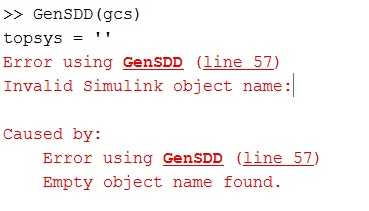
\includegraphics[scale=0.8]{errorIfUrunToolWithoutOpeningModel.jpg}}
		\caption{Error due to incorrect \mcode{gcs} value}
		\label{fig:error1}
	\end{figure}

	\subsection*{Error 2}
	In the example shown in Figure~\ref{fig:error2}, the \mcode{GenSDD} function was given the full path to a model on the user's computer system. 
	The problem is that \mcode{GenSDD} does not take the full path to a model on your computer system, but rather uses the full path within \simulink{} to a system within a given model (these paths are indicated in the address bar within \simulink{}).
	\begin{figure}\centering
		\fbox{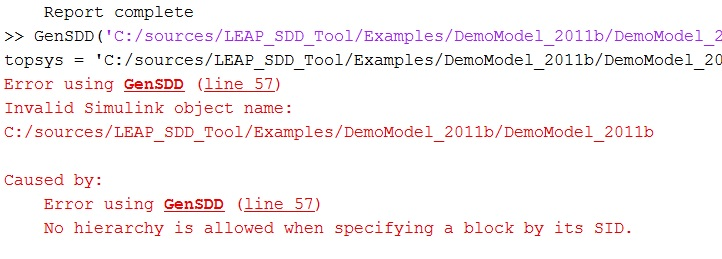
\includegraphics[width=\textwidth]{errorIfIenterPathRelative2myMachineNotSimulinkPath.jpg}}
		\caption{Error due to incorrect path}
		\label{fig:error2}
	\end{figure}
\end{document}